%%%%%%%%%%%%%%%%%%%% book_it.tex %%%%%%%%%%%%%%%%%%%%%%%%%%%%%
%
% Esempio di file principale per i capitoli della vostra  "monografia"
%
% Usare questo file come template per il vostro documento.
%
%%%%%%%%%%%%%%%% Springer-Verlag %%%%%%%%%%%%%%%%%%%%%%%%%%


% CONSIGLIATO
%%%%%%%%%%%%%%%%%%%%%%%%%%%%%%%%%%%%%%%%%%%%%%%%%%%
\documentclass[envcountsame,envcountchap]{svmono}

% scegliere le opzioni per []  come richiesto dalla lista 
% nella Reference Guide, Sez. 2.2

\usepackage{makeidx}         % permette di generare l'indice
\usepackage{graphicx}        % pacchetto grafico standard LaTeX 
                             % per l'inclusione di file immagine
\graphicspath{{./}{Figure/}}
\usepackage{amsfonts,amsmath,amssymb}
\usepackage{multicol}        % usato per l'indice a due colonne
\usepackage{subcaption}
\usepackage{cancel}
\usepackage{quoting}
\usepackage[bottom]{footmisc}% mette le note a pie' di pagina
\usepackage[italian]{babel}
\usepackage{mathtools}
% etc.
% si veda la lista di ulteriori pacchetti utili 
% nella Reference Guide, Sez. 2.3, 3.1-3.3

\def\theoremname{Teorema}
\makeindex             % usato per l'indice degli argomenti 
                       % si prega di usare lo stile svind.ist con 
                       % il vostro programma makeindex


%%%%%%%%%%%%%%%%%%%%%%%%%%%%%%%%%%%%%%%%%%%%%%%%%%%%%%%%%%%%%%%%%%%%%

\begin{document}

\author{Armenante Davide}
\title{Progetto di macchine\\
%{\small SPIN Springer internal project number, se noto}
}
\subtitle{Appunti del corso}
\date{2020}
\maketitle

\frontmatter%%%%%%%%%%%%%%%%%%%%%%%%%%%%%%%%%%%%%%%%%%%%%%%%%%%%%%

%%%%%%%%%%%%%%%%%%%%%%% dedic.tex %%%%%%%%%%%%%%%%%%%%%%%%%%%%%%%%%
%
% Esempio di dedica
%
% Usare questo file come template per il vostro documento.
%
%%%%%%%%%%%%%%%%%%%%%%%% Springer-Verlag %%%%%%%%%%%%%%%%%%%%%%%%%%

\thispagestyle{empty}
\vspace*{3.5cm}
\begin{flushright}

% scrivere qui
{\large Prego comunque...}

\end{flushright}




%%%%%%%%%%%%%%%%%%%%%% pref_it.tex %%%%%%%%%%%%%%%%%%%%%%%%%%%%%%%%%%%%%
%
% Esempio di prefazione
%
% Usare questo file come template per il vostro documento.
%
%%%%%%%%%%%%%%%%%%%%%%%% Springer-Verlag %%%%%%%%%%%%%%%%%%%%%%%%%%

\preface

Prima che il lettore si immerga in questa appassionante lettura vorrei fare due precisazioni. L'impaginazione è tanto figa quanto il libro è scritto male, diffidate, non si tratta di un elaborato professionale ma di appunti presi a lezione. Apprezzate però, tutte le immagini sono state rifatte vettorialmente. Si ringraziano\footnote{Non avevo voglia di dedicare una pagina intera ai ringraziamenti per scrivere due righe, gli alberi ringraziano} soprattutto i revisori Carlo Pini\footnote{Detto CP7} e Fausto Dicech.



\tableofcontents


\mainmatter%%%%%%%%%%%%%%%%%%%%%%%%%%%%%%%%%%%%%%%%%%%%%%%%%%%%%%%
% !TEX root = ../ProgettoMacchine2020.tex
% !TEX encoding = UTF-8 Unicode
% !TEX program = pdflatex
% !TEX spellcheck = it-IT
\chapter{Richiami teorici}
\section{Teoria della similitudine}
L’applicazione della teoria della similitudine costituisce un primo e potente strumento della progettazione, in particolar modo per quanto riguarda le turbomacchine. La teoria della similitudine permette di risolvere diversi problemi:
\begin{itemize}
\item[$-$] note le prestazioni di una macchina che ha determinate dimensioni,
si possono ricavare le prestazioni di una macchina geometricamente simile a quella considerata ma di diverse dimensioni nel dettaglio permette la realizzazione di prototipi in scala ridotta (esempio tipico: modellino della grande turbina idraulica che viene provato prima di procedere alla costruzione della macchina vera);
\item[$-$] nota una ben determinata condizione di funzionamento di una turbomacchina, come potrebbero essere le condizioni di progetto, si possono individuare altre condizioni di funzionamento ottenute variando la velocità di rotazione, la portata, oppure il lavoro scambiato (fluido/macchina);
\item[$-$] curve di prestazioni rilevate in determinate condizioni ambientali possono essere espresse in funzione di parametri che sono invarianti al variare delle condizioni ambientali stesse. Possiamo conoscere le prestazioni di una macchina operante in condizioni diverse (ad esempio un compressore sul livello del mare ad agosto e in montagna a Natale);
\end{itemize}
Accanto a tutti questi aspetti riguardanti la capacità di predire le prestazioni di una macchina, si ritrova anche un ausilio al designer in sede di progettazione. Con la teoria della similitudine si può stabilire in maniera semplice e veloce fin da subito quale sarà il tipo di macchina migliore da usare, quale sarà la sua geometria di base e quali le dimensioni generali. Grazie a ciò si riesce a sfruttare l’esperienza già maturata nella progettazione, sviluppo e test di altre macchine simili. Possedere un database ricco di informazioni relative a macchine pregresse risulta essere un vantaggio progettuale non di poco conto.


ll teorema di Buckingham (conosciuto anche come teorema pi greco), dovuto al fisico statunitense Edgar Buckingham, afferma:
\begin{quotation}
	Dato un problema descritto da un certo numero di equazioni in cui siano presenti $n$ variabili fisiche, se le dimensioni fondamentali di queste variabili sono $x$ allora il problema può essere completamente descritto da $n - x$ variabili adimensionali.
\end{quotation}
Per studiare il comportamento di una turbomacchina si definisce il seguente funzionale.
\begin{equation}
f(D_i,l_j,\dot{m},w,L_i,\mu,a_{01},\rho_{01})=0
\end{equation}
Con\\
$D_i$: serie di diametri rilevanti;\\
$l_j$: serie di lunghezze rilevanti;\\
$\dot{m}$: portata in massa;\\
$w$: velocità angolare;\\
$L_i$: lavoro ideale scambiato tra macchina e fluido per unità di massa;\\
$\mu$: viscosità dinamica del fluido;\\
$a_{01}$: velocità del suono all'ingresso in condizioni di ristagno;\\
$\rho_{01}$: densità del fluido.
\begin{equation}
Re= \frac{\rho_{01} w D^2}{\mu}
\end{equation}
\begin{equation}
Ma= \frac{w D}{a_{01}}
\end{equation}
Si evidenzia che tutti gli argomenti del funzionale sono descritti da una combinazione delle tre grandezze fondamentali M L T, ovvero massa lunghezza e tempo. Tenendo presente ciò è possibile adimensionalizzare gli argomenti del funzionale ottenendo una nuova espressione per lo stesso.

In una macchina termica in cui il fluido cambia le proprietà nei vari punti della macchina per definire la densità o la velocità del suono devo fissare
convenzionalmente una condizione rispetto alla quale vado a valutare quella
proprietà. 

Una condizione di riferimento che viene spesso adottata (non è
l’unica) potrebbe essere quella di valutare queste quantità nelle condizioni
totali all’ingresso della macchina (cioè condizioni valutate immaginando il fluido in quiete) che possiamo indicare con il pedice $01$ ($0$: condizioni totali o di ristagno; $1$: condizioni di ingresso).

<<<<<<< Updated upstream
Si può allo stesso modo definire le cifre di flusso $\varphi$ e di pressione $\psi$ andando ad adimensionalizzare rispettivamente la portata e il lavoro unitario:
=======
Si può allo stesso modo definire le cifre di flusso $\Phi$ e di pressione $\psi$ andando ad adimensionalizzare rispettivamente la portata e il lavoro unitario:
>>>>>>> Stashed changes
\begin{equation}
\varphi = \frac{\dot{m}}{\rho_{01}w D^3} \left( =\frac{Q}{w D^3} \right)
\end{equation}
\begin{equation}
\psi = \frac{L_i}{w^2 D^2}
\end{equation}
Il funzionale può essere espresso quindi secondo i numeri adimensionali:
\begin{equation}
f(\pi_i,\pi_j,\varphi,\psi,Re,Ma)=0
\end{equation}
Si può semplificare sotto le ipotesi di geometria simile.
\begin{equation}
f(\varphi,\psi,Re,Ma)=0
\end{equation}
Supponendo di confrontare due macchine se queste hanno le gli stessi valori di $\pi_i$ e $\pi_j$, allora la geometria tra le due macchine sarà da considerarsi simile e sotto queste ipotesi il funzionale si semplifica come di seguito:
\begin{figure}
\centering
  \includegraphics[width=\textwidth]{fig/moody.jpg}
\caption{}
\label{fig:moody}
\end{figure}
Guardando il diagramma di Moody in figura \ref{fig:moody}, in ascisse è presente $Re$ ed in ordinate il coefficiente di perdita di carico del nostro tubo $\xi$. Le scale sono logaritmiche. Il legame tra $\xi$ e $Re$, per bassi numeri di Reynolds, è rappresentato da una retta. Poi si ha una zona di transizione non ben definita ed infine una serie di linee a rugosità relativa costante $\epsilon/D$ (con $\epsilon$ rugosità media).

Nel primo tratto di legame lineare si ha una corrente laminare. Il tratto tratteggiato è un tratto nel quale, in condizioni sperimentali assolutamente controllate, è possibile mantenere un flusso laminare ma altamente instabile. In condizioni di flusso turbolento la perdita di carico dipende dalla rugosità.
Possiamo inoltre osservare che se consideriamo un solo valore di rugosità relativa la curva presenta una certa pendenza fino ad un certo valore di $Re$ (limite o critico) e poi diventa orizzontale. Sotto le ipotesi di moto turbolento pienamente sviluppato possiamo quindi trascurare l’influenza di Reynolds nel funzionale. Va ovviamente considerato che le rugosità relative di una macchina grande saranno in genere diverse da quelle che si possono ottenere con macchine piccole, quindi bisogna tenerlo presente. Variazioni anche grandi del numero di Reynolds, purché in regime di moto turbolento completamente sviluppato (corrispondenti a valori di Re molto elevati), non influenzano le prestazioni della mia macchina.

Se il numero di Reynolds è superiore ad un certo valore limite il coefficiente di perdita di carico è indipendente da $Re$. Se trasferiamo questa osservazione alla turbomacchina si può verificare sperimentalmente che se $Re$ è molto elevato questo potrà anche variare ma le prestazioni non ne saranno influenzate. Variazioni anche grandi del numero di Reynolds purché siano nel
campo di $Re$ molto elevato, non influenzano le prestazioni della mia macchina.
\begin{equation}
f(\varphi,\psi,Ma)=0
\end{equation}
In seguito, si aggiungerà una perdita sul modello in quanto il rendimento di una macchina piccola sarà sempre inferiore al rendimento di una macchina grande.

In ultimo se si considerano i fenomeni di comprimibilità trascurabili, si può trascurare anche il numero di Mach, equivalentemente si fa l'ipotesi $Ma\;<\;0.3$.
\begin{align*}
f(\varphi,\psi)=0
\end{align*}
Dotando la pompa di un sensore di pressione, giri e portata, posso andare a definire una curva di prestazione adimensionale.
Si definiscono orea le tre componenti del vettore velocità:
\begin{itemize}
\item[$c$]: velocità assoluta;
\item[$w$]: velocità relativa;
\item[$u$]: velocità periferica;
\end{itemize}
Naturalmente affinché le macchine operino in condizioni di similitudine devono, per definizione, avere $\varphi$ e $\psi$ uguali. 
\begin{equation}
\varphi=\frac{Q}{w D^3} \propto \frac{c_m}{u}
\end{equation}

\begin{equation}
\psi = \frac{L_i}{w^2 D^2} \propto \frac{c_u}{u}
\end{equation}
Quindi, assegnato $D$, la cifra di flusso è proporzionale alla velocità meridiana e inversamente proporzionale a $u$ dove $u= \omega \times r$. La variazione di $c_u$ corrisponde alla variazione dell'energia cinetica a valle della macchina. 

Mantenere $\varphi$ e $\psi$ uguali significa avere triangoli di velocità simili (vedi la figura \ref{fig:tria}).
\begin{figure}
\centering
  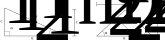
\includegraphics[width=.8\textwidth]{fig/triang.pdf}
\caption{}
\label{fig:tria}
\end{figure}
Consideriamo il caso di una macchina idraulica e vediamo come possiamo trovare il luogo dei punti di funzionamento simili sul piano delle prestazioni e quindi come le curve di prestazioni adimensionali stanno in rapporto con le curve di prestazioni dimensionali.

Se rileviamo le prestazioni di una pompa otteniamo la curva di funzionamento caratteristica (diagramma prevalenza-portata) per un certo valore della velocità di rotazione (figura \ref{fig:hq}).
\begin{figure}[h!]
\centering
  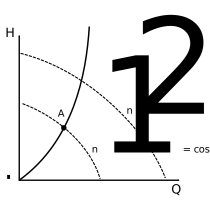
\includegraphics[width=.3\textwidth]{fig/hq.pdf}
\caption{}
\label{fig:hq}
\end{figure}
Queste sono curve espresse in funzione di grandezze dimensionali, ma andando ad adimensionalizzare si possono ottenere tali curve in funzione delle relative cifre di pressione e di flusso.  Si consideri un punto di funzionamento $A$, il luogo dei punti di funzionamento simili ad $A$ sarà caratterizzato dal fatto di avere stessi $\varphi$ e $\psi$.

Considerando quindi il generico punto $x$ posso scrivere
\begin{equation}
\varphi = \frac{Q}{w D^3}= \frac{Q_x}{w_x D^3}
\end{equation}
Considerando una macchina con lo stesso diametro posso scrivere
\begin{equation}
\frac{Q_x}{Q}=\frac{w_x}{w} \; \Rightarrow \; Q_x = Q \frac{w_x}{w}
\end{equation}
Imponendo invece l'uguaglianza della cifra di pressione
\begin{equation}
\psi = \frac{gH}{w^2 D^2}= \frac{gH_x}{w_x^2 D^2}
\end{equation}
In questo modo si ottiene
\begin{equation}
H_x = H(\frac{w_x}{w})^2 = H(\frac{Q_x}{Q})^2 \Rightarrow H_x = \frac{H}{Q^2}Q_x^2
\end{equation}
Che è l'equazione di una parabola sul piano H-Q, passante per il punto A e per l'origine degli assi. 
Noto che il lavoro varia al variare del quadrato della velocità angolare mentre la portata varia linearmente. 
Ad ogni curva $\varphi - \psi$ corrisponde una curva di rendimento, posso quindi individuare una coppia $\bar{\varphi} - \bar{\psi}$ ottimale (figura \ref{fig:adim}).
\begin{figure}[h!]
\centering
  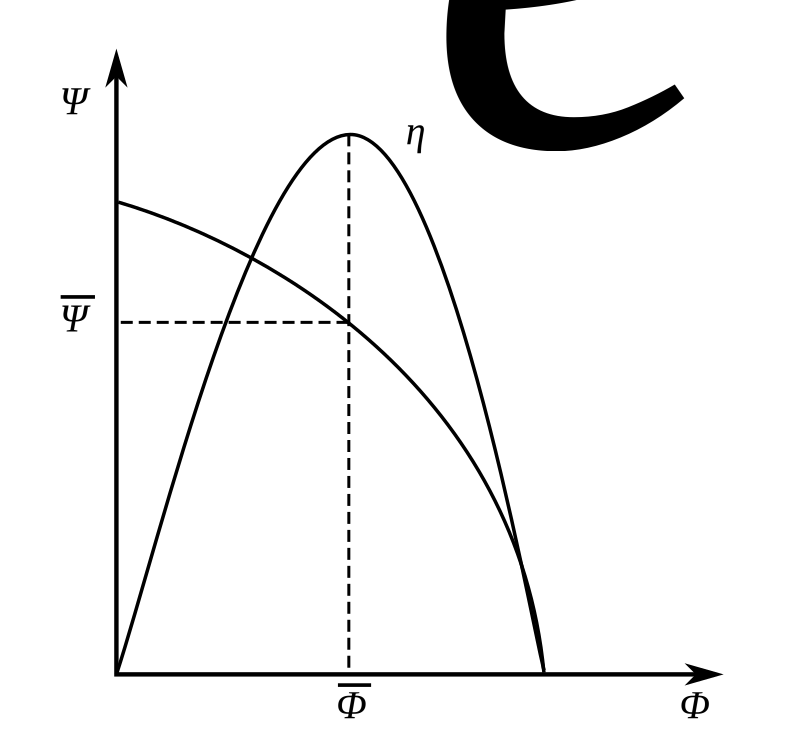
\includegraphics[width=.3\textwidth]{fig/adim.pdf}
\caption{}
\label{fig:adim}
\end{figure}
Posso anche definire il coefficiente di velocità periferica.
\begin{equation}
k_P = \frac{w D}{\sqrt{L_i}}
\end{equation}
Si tratta di una cifra che lega la velocità periferica della macchina al lavoro ideale della stessa.

Quando ho $\varphi$ e $\psi$ posso definire una cifra di potenza adimensionalizzata come prodotto delle due.
\begin{equation}
\Lambda = \frac{P_e}{\rho w^3 D^5}
\end{equation}
Per macchina motrice
\begin{equation}
\Lambda = \varphi \psi \eta_e
\end{equation}
Per macchina operatrice
\begin{equation}
\Lambda = \frac{\varphi \psi}{\eta_e}
\end{equation}
Con la seguente espressione posso poi eliminare la caratteristica geometrica ottenere il numero specifico di macchina (o velocità specifica) che rappresenta una condizione di funzionamento lavoro-portata indipendente dalla dimensione della macchina. 
\begin{equation}
w_s = k = \varphi^{1/2} \psi^{-3/4} = w \frac{\sqrt{Q}}{L_i^{3/4}}
\end{equation}
<<<<<<< Updated upstream
La forma della macchina varierà al variare di k . Avere dei k piccoli significa avere delle macchine nelle quali il termine di scambio di energia è prevalente rispetto al termine di portata. Questo numero permette, grazie all'esperienza storica (ovvero di tutti i dati che il progettista o la sua azienda possiedono in merito alle prestazioni di altre macchine), di classificare la forma geometrica di una macchina in base alle condizioni portata - lavoro.
=======
La forma della macchina varierà al variare di k . Avere dei k piccoli significa avere delle macchine nelle quali il termine di scambio di energia è prevalente rispetto al termine di portata. Questo numero permette, grazie all’esperienza storica (ovvero di tutti i dati che il progettista o la sua azienda possiedono in merito alle prestazioni di altre macchine), di classificare la forma geometrica di una macchina in base alle condizioni portata - lavoro.
>>>>>>> Stashed changes
\begin{figure}[h!]
\centering
  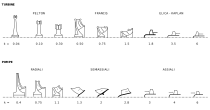
\includegraphics[width=\textwidth]{fig/numcar.pdf}
\caption{Variazione della forma delle giranti delle turbine idrauliche al variare del numero caratteristico di macchina.}
\label{fig:numcar}
\end{figure}
Queste cifre sono funzioni di k. Possono allora essere definite delle curve che riportano in ascissa il valore del numero caratteristico k e sulle ordinate i valori dei 4 rapporti.
Sfruttando l'esperienza possiamo analizzare le migliori macchine esistenti e vedere
quanto valgono per quelle macchine le cifre adimensionali $\pi_i$ , $\pi_j$ e diagrammarle in funzione di k . Facciamo un esempio concreto considerando una tipica macchina radiale (una pompa centrifuga) e consideriamo la sezione meridiana semplificata al massimo (figura \ref{fig:pala}).
\begin{figure}
\centering
\begin{minipage}{.5\textwidth}
  \centering
  \includegraphics[width=.9\linewidth]{fig/pala.pdf}
  \captionof{figure}{}
  \label{fig:pala}
\end{minipage}%
\begin{minipage}{.5\textwidth}
  \centering
  \includegraphics[width=.6\linewidth]{fig/primo_1.pdf}
  \captionof{figure}{}
  \label{fig:primo_1}
\end{minipage}
\end{figure}
Si definiscono le seguenti dimensioni caratteristiche più significative. Si tratta di un esempio didattico, in realtà posso andare a definire un database molto più ampio e raffinato. Siano
\begin{itemize}
\item[-]$D_2$: diametro massimo della girante;\\
\item[-]$D_1$: diametro massimo della sezione di ingresso;\\
\item[-]$D_1^{'}$: diametro minimo della sezione d'ingresso;\\
\item[-]$b_2$: altezza della pala in uscita;\\
\item[-]$b_1$: altezza della pala in ingresso.
\end{itemize}
Per definire $b_1$ bisogna prendere il diametro medio e con riferimento al punto di intersezione tra questo ed il profilo della pala in ingresso si traccia la circonferenza inscrivibile nella sezione d’ingresso. Come grandezza caratteristica della sezione d’ingresso prendo proprio il diametro di questa circonferenza.
Per queste grandezze posso definire le seguenti cifre adimensionali:
\begin{align*}
\frac{D_1}{D_2} \; \; \; \frac{D_1^{'}}{D_2} \; \; \; \frac{b_1}{D_2} \; \; \; \frac{b_2}{D_2} 
\end{align*}
Queste cifre sono funzioni di $k$. Posso allora essere definite delle curve che riportano in ascisse il valore del numero caratteristico $k$ ed in ordinate i valori dei 4 parametri.
Naturalmente fissato $k$ devo poi determinare il numero di giri a cui deve lavorare la macchina. 
Ricapitolando, note portata, prevalenza e fissata la velocità di rotazione, conosco il valore di $k$. Entrando in questi diagrammi si trovano i valori dei quattro parametri e quindi definisco per sommi capi la sezione meridiana della nostra macchina (figura \ref{fig:primo_1}).

Esiste una dimensione ottimale cioè una dimensione alla quale corrisponde il massimo rendimento. Bisogna però definire un’ulteriore grandezza detta diametro specifico.
\begin{equation}
D_s= \varphi^{-1/2} \psi^{1/4} = D \cdot \frac{L_i^{1/4}}{\sqrt{Q}}
\end{equation}
Bisogna cercare di eliminare la velocità di rotazione. È stato verificato che esiste, con riferimento alle dimensioni di massimo rendimento, un legame tra $D_s$ e $w_s$. 
\begin{equation}
D_s=f(w_s)
\end{equation}
Questa funzione è descritta empiricamente sul \textit{Diagramma di Cordier}. Questo diagramma rappresenta l’interpolazione di una serie di dati sperimentali (da vedere come correlazione statistica).
Grazie alle curve di Balié è possibile osservare l’entità delle variazioni che si ottengono andando a discostarsi, entro certi limiti, dalla curva di Cordier.
Si può estendere questa relazione con i diagrammi di Baliè, intorno alla curva si disegnano curve di isorendimento.
\begin{figure}
\centering
\begin{minipage}{.5\textwidth}
  \centering
  \includegraphics[width=.95\linewidth]{fig/cord_diag.pdf}
  \captionof{figure}{Diagramma di Cordier}
  \label{fig:cord_diag}
\end{minipage}%
\begin{minipage}{.5\textwidth}
  \centering
  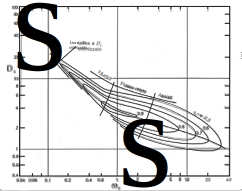
\includegraphics[width=.95\linewidth]{fig/primo_3.pdf}
  \captionof{figure}{}
  \label{fig:primo_3}
\end{minipage}
\end{figure}

\section{Influenza di Re}
Queste considerazioni sono state fatte trascurando l'influenza di Re. Ricordando il diagramma di Moody la relazione è fatta rispetto a $\epsilon/D$. Per le macchine è essenzialmente uguale, al diminuire di Re le curve si spostano più in basso, questo effetto si riflette in un abbassamento di rendimento e quindi di prevalenza.

Questo è un fenomeno prevedibile in termini statistici, storicamente grazie all'accumulazione di dati sono stati definiti due fattori di correzione, di rendimento $f_\eta$ e $f_\psi$ diagrammati rispetto a $Re$. Man mano che $Re$ scende il loro effetto diventa sempre più importante. 
\begin{figure}
\centering
\begin{minipage}{.4\textwidth}
  \centering
  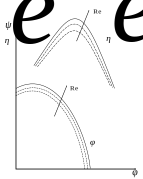
\includegraphics[width=.95\linewidth]{fig/secondo_1.pdf}
  \captionof{figure}{}
  \label{fig:secondo_1}
\end{minipage}%
\begin{minipage}{.6\textwidth}
  \centering
  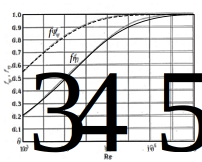
\includegraphics[width=.95\linewidth]{fig/secondo_2.pdf}
  \captionof{figure}{}
  \label{fig:secondo_2}
\end{minipage}
\end{figure}

Parto dalla $w_s$, scrivo $\varphi$ e $\psi$ nei diversi punti di funzionamento della macchina in funzione di $w_s$ ($\equiv k$). 
\begin{align*}
w_s= \varphi^{1/2}\psi^{-3/4} \Rightarrow 
\begin{cases}
\psi = \psi(w_s)\\
\eta = \eta(w_s)
\end{cases}
\Rightarrow
\begin{cases}
f_{\psi} = f(Re)\\
f_{\eta} = f(Re)
\end{cases}
\end{align*}
Con i coefficienti correttivi vado a trovare le cifre adimensionali corrette \begin{align*}
\begin{cases}
\psi_{corretto} = f_{\psi} \cdot \psi(w_s)\\
\eta_{corretto} = f_{\eta} \cdot \eta(w_s)
\end{cases}
\end{align*}
A questo punto è possibile procedere a ritroso. Trovato il valore corretto avrò
\begin{align*}
\omega_s = \varphi^{1/2} \psi^{-3/4} =  \varphi_{corretto}^{1/2} \psi_{corretto}^{-3/4} = cost
\end{align*}
partendo proprio dalla definizione di $\omega_s$ è possibile costruire le curve di prestazione corrette.

\section{Effetto scala}
Si considera poi un effetto scala non solo legato alle rugosità superficiali ma anche legato ai giochi. L'effetto scala può essere espresso rispetto ai rapporti dimensionali. Queste relazioni sono sempre costruite per via empirica sulla base dei dati storici.

A parità di bontà di progettazione, geometria, ecc... la macchina grande ha un rendimento maggiore rispetto alla macchina piccola. Questo si spiega facendo due osservazioni: a parità di tecnologia produttiva è possibile ritenere costante il valore della rugosità superficiale delle palettature della girante. In una macchina grande la rugosità relativa sarà quindi più bassa, quindi le perdite di carico saranno superiori nella macchina piccola. In secondo luogo bisogna tener conto dei giochi presenti tra parte fissa e parte mobile, che non possono scendere al di sotto di un certo limite. Nelle macchine grandi questi diventeranno trascurabili. 
\begin{figure}
\centering
  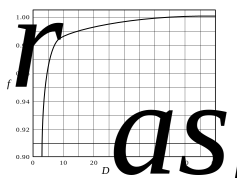
\includegraphics[width=.5\textwidth]{fig/dDchart.pdf}
\caption{}
\label{fig:dDchart}
\end{figure}

Facendo riferimento alle pompe possiamo definire un rapporto dimensionale 
\begin{align*}
\frac{D_1}{D_2} \triangleq  \mbox{Rapporto di scala}, \; D_1 < D_2
\end{align*}
In riferimento alla figura \ref{fig:dDchart} rendimento si può esprimere come
\begin{align*}
\eta = \eta_S \cdot f_r(D)
\end{align*}
E la relazione tra il rendimento tra le pompe di scala diversa è il seguente
\begin{equation}
\frac{1-\eta_1}{1-\eta_2} = \left( \frac{D_2}{D_1}\right)^\alpha
\end{equation}
La stessa operazione viene fatta per le turbine idrauliche
\begin{align*}
\frac{1-\eta_1}{1-\eta_2} = \left[ \frac{Re_{u,2}}{Re_{u,1}} \right]^n, \; \; n=0.1 \div 0.25
\end{align*}
\begin{align*}
\frac{1-\eta_1}{1-\eta_2} =0.5 + 0.5 \left[ \frac{Re_{u,2}}{Re_{u,1}} \right]^{0.2}
\end{align*}
\begin{align*}
\frac{1-\eta_1}{1-\eta_2} = 0.3 + 0.7 \left[ \frac{Re_{u,2}}{Re_{u,1}} \right]^{0.2} \; \to \; \mbox{Turbine Kaplan}
\end{align*}
\section{Flusso comprimibile}
Se si considera il flusso comprimibile le relazioni diventano più complesse. Infatti si ha:
\begin{equation}
\psi=f(\varphi,Ma)
\end{equation}
$\psi$ dipende quindi anche dal numero di Mach. 
Nel diagramma $\varphi-\psi$ si ottengono diverse curve al variare del numero di Mach (Figura \ref{fig:ComprMach}), le curve diventano di difficile lettura e comprensione.Infatti, per diversi valori delle grandezze termodinamiche di temperatura e pressione risulta possibile ottenere le stesse quantità di lavoro unitario, e ciò comporta una mancata definizione univoca dello stesso. Si tratta di una rappresentazione poco fisica e di un esercizio esclusivamente accademico.
\begin{figure}[h!]
\centering
  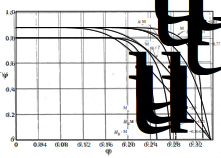
\includegraphics[width=.85\textwidth]{fig/ComprMach.pdf}
\caption{Curve adimensionali di funzionamento di una famiglia di compressori, per un fluido assegnato, a diversi numeri di Mach periferici. Sono definiti $Ma = \frac{w \frac{D}{2}}{a_{01}}$, $Mu = \frac{w \frac{D}{2}}{a}$}
\label{fig:ComprMach}
\end{figure}
Per questo tipo di macchine si utilizzeranno curve molto diverse. Per avere una grandezza confrontabile di funzionamento devo effettuare tutte le prove in condizioni standard. In questo modo posso rappresentare condizioni di funzionamento in modo univoco. 
Definisco il significato dei pedici:
\begin{itemize}
\item $s$: grandezze relative alle condizioni standard;
\item $c$: valori corretti, cioè riportati alle condizioni standard;
\item ``  ": valori da correggere rilevati nel corso della prova.
\end{itemize}
Si elencano di un gas generico miscela di due gas con massa molare $M$\footnote{Nota bene: solo in questo contesto si utilizza $M$ per indicare la massa molare, in tutto il resto del libro viene usato per indicare il numero di Mach}
\begin{align*}
\frac{p}{\rho} = \frac{p_1}{\rho} + \frac{p_2}{\rho} = x_1  \frac{p_1}{\rho_1} + x_2  \frac{p_2}{\rho_2} = RT \left( \frac{x_1}{M_1} + \frac{x_2}{M_2} \right) = RT(\frac{1}{M_{tot}})
\end{align*}
\begin{align*}
c_p = x_1 c_{p1} + x_2 c_{p2}
\end{align*}
\begin{align*}
\cfrac{\gamma}{\gamma -1} = \cfrac{\cfrac{x_1}{M_1} \cfrac{\gamma_1}{\gamma_1 -1}+\cfrac{x_2}{M_2} \cfrac{\gamma_2}{\gamma_2 -1}}{\cfrac{x_1}{M_1}+\cfrac{x_2}{M_2}}
\end{align*}
Con $M_{1,2,tot}$ numero di moli, $x_{1,2}$ frazione molare e $R$ costante dei gas perfetti. Si ricorda poi che definiti calore specifico a pressione costante $c_p$ e calore specifico a volume costante $c_v$ si ha
\begin{align*}
\gamma = \frac{c_p}{c_v}, \;\;\; R = c_p - c_v
\end{align*}

Di seguito vengono riportate le grandezze significative corrette rispetto alle condizioni standard.\\
Rapporto di compressione corretto rispetto alle condizioni ambientali standard:
\begin{align*}
\frac{p_{02}}{p_{01}} = \frac{p_{01c}}{p_{01s}} \; \Rightarrow \; p_{02c} = p_{02}\frac{p_{01s}}{p_{01}}
\end{align*}
Parametro di portata
\begin{align*}
\frac{\dot{m}\sqrt{T_{01}}}{p_{01}}=\frac{\dot{m_c}\sqrt{T_{01s}}}{p_{01s}} \; \Rightarrow \; \dot{m_c} = \dot{m} \sqrt{\frac{T_{01}}{T_{01s}}} \bigg(\frac{p_{01s}}{p_{01}} \bigg)
\end{align*}
Parametro di velocità
\begin{align*}
\frac{n}{\sqrt{T_{01}}}=\frac{n_c}{\sqrt{T_{01s}}} \; \Rightarrow \; n_c = n \sqrt{\frac{T_{01s}}{T_{01}}}
\end{align*}
Si definiscono quindi le condizioni ambientali standard.
Pressione ridotta
\begin{align*}
\delta = \frac{p_{01}}{p_{01s}}
\end{align*}
Temperatura ridotta
\begin{align*}
\theta = \frac{T_{01}}{T_{01s}}
\end{align*}
Si possono esprimere più sinteticamente le grandezze corrette:
\begin{align*}
p_{01c} = \frac{p_{02}}{\delta}
\end{align*}
\begin{align*}
\dot{m_c}= \dot{m} \frac{\sqrt{\theta}}{\delta}
\end{align*}
\begin{align*}
n_c = \frac{n}{\sqrt{\theta}}
\end{align*}
\begin{figure}
\centering
  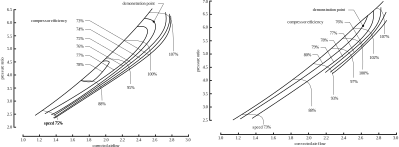
\includegraphics[width=\textwidth]{fig/CompMaps.pdf}
\caption{}
\label{}
\end{figure}
Si ottiene così la portata di massa corretta e il numero di giri corretto.
In questo modo si trovano le mappe di funzionamento delle macchine. Si diagrammano la portata d'aria corretta con il rapporto di compressione. Sono tracciate diverse curve al variare dei giri con le curve di isorendimento.

A questo punto si espande l'espressione di $\varphi$ tenendo conto delle seguenti espressioni di $M_{01}$, $p$ e $a$
\begin{align*}
M_{01}=\frac{w D}{a_{01}}= \frac{w D}{\sqrt{k R T_{01}}}, \;\;\;p = \rho_i RT, \;\;\; a = \sqrt{k R T}
\end{align*}
\begin{equation}
\varphi = \frac{\dot{m}}{\rho_{01} w D^3} = \frac{\dot{m}}{\rho_{01} M_{01} a_{01} D^2} = \frac{\dot{m} R T_{01}}{\rho_{01} M_{01} \sqrt{k R T_{01}} D^2} = \frac{\dot{m} \sqrt{R T_{01}}}{\rho_{01} M_{01} \sqrt{k} D^2}
\end{equation}
Mentre la cifra $\psi$ è esprimibile in funzione dei soli $M_{01}$, rapporto di compressione e delle caratteristiche del fluido ($k$)
\begin{equation}
\psi = \cfrac{L_i}{w^2 D^2} = \cfrac{\Delta h_{0s}}{w^ 2 D^2} = \cfrac{\cfrac{k}{k-1} R T_{01}\left[ \bigg( \cfrac{p_{02}}{p_{01}} \bigg)^{\frac{k-1}{k}}-1\right]}{M_{01}^2 k R T_{01}} = \cfrac{\cfrac{1}{k-1} \left[ \bigg( \cfrac{p_{02}}{p_{01}} \bigg)^{\frac{k-1}{k}}-1\right]}{M_{01}^2 }
\end{equation}

L'idea è quella di rappresentare in modo univoco il comportamento del compressore usando i termini $\varphi$, $\psi$ ma mantenendo la significatività fisica.

Se utilizzo lo stesso fluido posso trascurare $R$ e $k$. Utilizzando la stessa macchina trascuro anche $D$, riferendosi alle condizioni standard posso considerare $M_{01}=cost$. Sotto le precedenti ipotesi ottengo le seguenti relazioni semplificate:
\begin{align*}
M_{01} \to \frac{w D}{\sqrt{R T_{01}}} \Rightarrow M_{01} \to \frac{w}{\sqrt{T_{01}}}
\end{align*}
\begin{align*}
\varphi \to \frac{\dot{m} \sqrt{RT_{01}}}{\rho_{01} D^2} \Rightarrow \varphi \to \frac{\dot{m} \sqrt{T_{01}}}{\rho_{01}}
\end{align*}
\begin{align*}
\psi \to \frac{p_{02}}{p_{01}}
\end{align*}
Si tratta di grandezze che posso andare a misurare in un banco prova. 
La mappa di funzionamento del compressore assume quindi una forma più leggibile, sull'asse delle ascisse ho la portata in massa corretta con la temperatura in ingresso e sulle ordinate il rapporto di compressione. Assieme a queste posso anche costruire le linee di isorendimento  e quindi la curva ideale operativa del compressore data dall'inviluppo delle curve di isorendimento.
\begin{figure}
\centering
  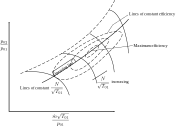
\includegraphics[width=.8\textwidth]{fig/secondo_8.pdf}
\caption{}
\label{fig:secondo_8}
\end{figure}
Guardando al diagramma in figura \ref{fig:secondo_8} si vede che abbiamo un fenomeno noto come ingolfamento del compressore, in particolare si vede dalle linee a velocità costante che tendono a diventare verticali in prossimità delle condizioni di ingolfamento . Intendiamo il raggiungimento di quella condizione di funzionamento in cui non è più possibile variare la portata variando il rapporto delle pressioni attorno alla macchina.
Questo perchè in qualche punto si raggiungono le condizioni di flusso sonico e quindi, ricordando lo studio dell'ugello convergente-divergente, abbiamo un
blocco sonico delle portata.

L'obiettivo è quello di lavorare il più possibile vicino alla ``operating line" che è la zona di massimo rendimento, il problema è che ci si trova pericolosamente vicino alla ``surge line". Oltre la surge line si innesca il fenomeno del pompaggio che può compromettere la macchina e l'impianto irrimediabilmente.

Riassumendo, nel comprimibile, operativamente si descrive il funzionamento delle turbomacchine non rispetto alle cifre di flusso e pressione, bensì attraverso nuove cifre più significative in questo contesto.
\section{Richiamo di termodinamica}
Lo scambio termico è trascurabile per i bassi tempi di residenza del fluido nel condotto, per questo motivo si considera il rotore adiabatico.

In un rotore adiabatico, per il primo principio della termodinamica, essendo il flusso di calore nullo, il lavoro è dato dal salto entalpico tra gli stati $1$ e $2$
\begin{equation}
L_{12}^{'} = h_{t1}-h_{t2}
\end{equation}
\begin{equation}\label{eq:ent_tot}
h_t=h+\frac{c^2}{2}+gz
\end{equation}
Con: 
$h_t$: entalpia totale\\
$h$: entalpia statica\\
$c^2/2$: quota cinetica\\
$gz$: quota gravitazionale\\[2mm]
Per una macchina motrice\footnote{Nel caso delle macchine operatrici si invertono i pedici $1$ e $2$ così da avere lavori per convenzione sempre positivi} si può scrivere
\begin{equation}\label{eq:L12}
L_{12}^{'} = \begin{cases} u_1 c_{u1}-u_2 c_{u2}\\
\cfrac{c_1^2-c_2^2}{2}+\cfrac{u_1^2-u_2^2}{2}-\cfrac{w_1^2-w_2^2}{2} \end{cases}
\end{equation}

Naturalmente il lavoro è stato scritto, in base alle note convenzioni, per una macchina motrice.

Il lavoro è costituito da una parte cinetica e da una parte statica, il che si può osservare confrontando le espressioni di $L_{12}^{'}$ nelle formule \ref{eq:ent_tot} e \ref{eq:L12}, in particolare la quota parte cinetica dipende dalla componente assoluta della velocità ($c$), mentre quella statica dipende dalle componenti assiale ($u$) e relativa ($w$).

Dato che in una macchina puramente assiale si conserva l'omonima componente u della velocità ( $u = cost$ ), allora il contributo $u_1^2 - u_2^2$ nell'espressione del lavoro è nullo: per questo una macchina radiale a parità di numero di stadi e condizioni, elabora più lavoro di una assiale, in quanto $u_1^2 - u_2^2$ è maggiore di zero.

Ponendomi come osservatore relativo rispetto al rotore eguagliando le due espressioni per il lavoro posso scrivere
\begin{equation}
u_1 c_{u1} - u_2 c_{u2} = h_1 + \frac{c_1^2}{2}+gz_1-h_2-\frac{c_2^2}{2}-gz_2
\end{equation}
Posso quindi definire la rotalpia\footnote{Grandezza che rappresenta l'entalpia totale del moto relativo} come grandezza di stato ed è tale, proprio in virtù dell'adiabaticità del rotore, e quindi per la conservazione dell'energia vale:
\begin{equation}
h+\frac{c^2}{2}+gz-u c_u = cost. = I
\end{equation}

Riassumendo:
\begin{itemize}
\item $I=cost.$ in un rotore adiabatico;
\item $h_t=cost.$ in uno statore adiabatico.
\end{itemize}

Posso esprimere tutte le grandezze fin'ora viste in un piano $T-s$ o $h-s$.

\section{Rendimenti per i compressori}
Si riporta la trattazione dei rendimenti fatta per i compressori, i concetti riportati valgono anche per le turbine, cambia solamente le convenzione nei segni. La seguente trattazione è un estratto del libro Macchine a fluido, ISBN 978-88-251-7397-0. 

Il rendimento è definito qualitativamente come il rapporto tra l'effetto utile ed il lavoro svolto dalla macchina. Sul lavoro svolto non ci sono ambiguità mentre in merito all'effetto utile si possono avere diverse formulazioni. Il lavoro utile può essere preso come il salto entalpico associato al rapporto di compressione tra le pressioni statiche o totali ingresso-uscita, oppure come combinazione tra grandezze statiche e totali tra ingresso e uscita. Le diverse definizioni di rendimento sono sostanzialmente da imputare alle quote cinetiche ingresso/uscita che possono essere contate o meno come effetto utile.
\begin{figure}
\centering
  
\includegraphics[width=.5\textwidth]{fig/schieraTComp.pdf}
\caption{}
\label{fig:schieraTComp}
\end{figure}
Con riferimento alla trasformazione termodinamica, trascurando i contributi cinetici all'ingresso e all'uscita, si possono definire il rendimento adiabatico ed il rendimento politropico. Tale approccio è spesso utilizzato quando non si vuole entrare nel dettaglio della macchina come invece è necessario fare quando si vogliono studiare le prestazioni dei singoli stadi. 

Nel caso di rendimento adiabatico, definendo con $l_{is}$ il lavoro lungo la trasformazione isoentropica e con $l_r$ quello lungo l'adiabatica reale e facendo riferimento alla \ref{fig:Rend1}, la definizione diventa
\begin{align*}
\eta_{ad} = \frac{h_{2'} - h_1}{h_2 - h_1} = \frac{c_p \left( T_{2'} - T_1 \right)}{c_p \left( T_2 - T_1 \right)} = \frac{\left( \beta^{\cfrac{\gamma -1}{\gamma}} -1 \right)}{\left( \beta^{\cfrac{n -1}{n}} -1 \right)} = \frac{l_{is}}{l_r}
\end{align*}
Avendo assunto $c_p = cost$ con la temperatura e pressione, ed essendo $\gamma$ l'indice dell'isoentropica ed $n$ quello della politropica corrispondente alla trasformazione reale. La scelta di questa definizione, oltre al facile utilizzo, è quella di fornire una indicazione diretta dello scostamento della trasformazione da quella migliore possibile che è l'isoentropica, senza dedicare particolare attenzione alle energie cinetiche presenti all'interno del sistema macchina.
\begin{figure}
\centering
\begin{minipage}{.45\textwidth}
  \centering
  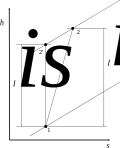
\includegraphics[width=.9\linewidth]{fig/Rend1.pdf}
  \captionof{figure}{}
  \label{fig:Rend1}
\end{minipage}%
\begin{minipage}{.55\textwidth}
  \centering
  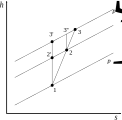
\includegraphics[width=.9\linewidth]{fig/Rend2.pdf}
  \captionof{figure}{}
  \label{fig:Rend2}
\end{minipage}
\end{figure}
Un'altra applicazione è il rendimento politropico che assume la trasformazione politropica reversibile tra i punti $1$ e $2$ come riferimento per la trasformazione reale. Tale assunzione viene incontro alla necessità, nel caso di macchine multistadio - o a singolo stadio ma con elevato rapporto di compressione - di non imputare ad una porzione di trasformazione la storia dei volumi specifici precedenti ed in particolar modo le irreversibilità precedenti. Con riferimento alla \ref{fig:Rend2}, dividendo la trasformazione in 3 porzioni, l'ultima parte della compressione richiede un salto entalpico pari a $\Delta h_r = h_3 - h_2$ che può essere confrontato con $\Delta h_{is} = h_{3'} - h_{2'}$ oppure con $\Delta h_is = h_{3''} - h_2$ a seconda dell'analisi che si vuole compiere sulla macchina.

Qualora si voglia analizzare il singolo stadio, o la singola porzione di trasformazione, allora appare corretto confrontare il salto reale con quello tra i punti $3''$ e $2$ in quanto più attinente alla trasformazione reale oggetto dell'attenzione. A causa della divergenza delle isobare il salto entalpico $3''$ e $2$ risulta maggiore di quello $3'$ e $2'$, dando luogo ad un rendimento maggiore. Se tale ragionamento viene esteso a porzioni infinitesime di compressione ci si avvicina alla definizione di rendimento politropico.

La scelta della trasformazione politropica reversibile - che tiene conto al suo interno di un riscaldamento del fluido operato da una sorgente esterna ma equivalente a quello causato dalle irreversibilità - consente di evidenziare il solo contributo delle irreversibilità e cioè del termine $\int Tds$.

Considerata allora la trasformazione 1-2, chiamato $l_p$ il lavoro lungo la politropica reversibile e $l_r$ il lavoro lungo la trasformazione adiabatica reale, il rendimento assume la seguente forma
%\begin{align*}
%\eta_p = \frac{l_p}{l_r} = \frac{\frac{nRT_1}{n-1} \left[ \left( \frac{p_2}{p_1} \right)^{\frac{n-1}{n} -1 \right]}{\frac{ \gamma RT_1}{\gamma-1} \left[ \left( \frac{p_2}{p_1} \right)^{\frac{n-1}{n} -1 \right]} = \frac{n}{\gamma} \frac{\gamma -1}{n -1}
%\end{align*}
Confrontando i due rendimenti a pari rapporto di compressione si vede come la differenza tra rendimento politropico e adiabatico aumenti al crescere del rapporto di compressione e che il rendimento adiabatico è sempre minore del politropico.
\begin{figure}
\centering
\begin{minipage}{.45\textwidth}
  \centering
  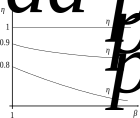
\includegraphics[width=.9\linewidth]{fig/Rend3.pdf}
  \captionof{figure}{}
  \label{fig:Rend3}
\end{minipage}%
\begin{minipage}{.55\textwidth}
  \centering
  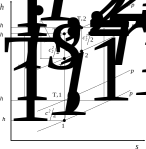
\includegraphics[width=.9\linewidth]{fig/Rend4.pdf}
  \captionof{figure}{}
  \label{fig:Rend4}
\end{minipage}
\end{figure}
Infatti poichè $\eta_p = l_p / l_r$ e $\eta_{ad} = l_{is} / l_r$, si ottiene
\begin{align*}
\eta_{ad} = \eta_p \frac{l_is}{l_r} = \eta_p \frac{\frac{\gamma}{\gamma-1} \left(\beta^{\frac{\gamma -1}{\gamma}}-1 \right)}{\frac{n}{n-1} \left(\beta^{\frac{n -1}{n}}-1 \right)}
\end{align*}
ed essendo $l_p$> $l_{is}$ si ottiene $\eta_{ad} < \eta_p$. Al fine di evidenziare al differenza tra le due trasformazioni è possibile definire il lavoro di controrecupero definito come
\begin{align*}
f = \frac{l_p - l_{is}}{l_{is}} = \frac{l_p}{l_{is}} -1 = \eta_p \frac{\left( \beta^{\frac{n-1}{n}} -1 \right)}{\left( \beta^{\frac{\gamma-1}{\gamma}} -1 \right)} -1 = \frac{\eta_p}{\eta_{ad}} -1
\end{align*}
Al crescere della differenza tra i due rendimenti, il fattore di controrecupero aumenta. Tale fattore è sempre maggiore di zero e si annulla quando i due rendimenti sono uguali, cioè quando non ci sono effetti termici sulla densità come avviene per le macchine idrauliche.

Qualora si voglia studiare gli effetti delle quote cinetiche, è possibile definire diversi tipi di rendimento, sempre definiti nella scia del rendimento adiabatico, denominati "total to total" e "total to static". Con riferimento alla \ref{fig:Rend4} si definiscono
\begin{itemize}
\item Rendimento total to total
\begin{align*}
\eta_{T,T} = \frac{\Delta h_{T,is}}{\Delta h_T} = \frac{h_{T,2'} - h_{T,1}}{h_{T,2} - h_{T,1}} = \frac{h_{2'} - h_1 + \left( \frac{c_2^2 - c_1^2}{2} \right)}{h_2 - h_1 + \left( \frac{c_2^2 - c_1^2}{2} \right)} = \frac{h_{2'} - h_1 + \left( \frac{c_2^2 - c_1^2}{2} \right)}{l_r} = \frac{l_{is}}{l_r}
\end{align*}
\item Rentimento Total to Static
\begin{align*}
\eta_{T,S} = \frac{h_{2'} - h_{T,1}}{h_{T,2} - h_{T,1}} = \frac{h_{2'} - h_1 - \left( \frac{ c_1^2}{2} \right)}{h_2 - h_1 + \left( \frac{c_2^2 - c_1^2}{2} \right)} = \frac{h_{2'} - h_1 + \left( \frac{c_2^2 - c_1^2}{2} \right)}{l_r} = \frac{l_{is}}{l_r}
\end{align*}
\end{itemize}
\pagebreak


\chapter{Turbine a flusso assiale e misto}
Le principali caratteristiche e differenze delle turbine a flusso assiale e misto rispetto i compressori assiali sono:
\begin{itemize}
	\item non si parlerà più di flusso assiale puro in quanto è presente anche una significativa componente radiale;
	\item il salto entalpico per stadio è di gran lunga superiore all'analogo elaborabile da un compressore;	
	\item entalpia e temperatura decrescono molto rapidamente; di conseguenza l'ipotesi di avere densità costante e l'andamento delle pressioni a gradino tra stadi successivi, non è più accettabile a causa proprio della dimensione del salto entalpico;
	\item sono presenti temperature molto elevate;
	\item si realizzano deflessioni importanti che vanno dai $50^{\circ}$ ai $180^{\circ}$;
	\item nel compressore la qualità del design del profilo è dominante mentre nella turbina il limite costruttivo è dato dai materiali della palettatura in quanto devono sopportare temperature e stress dovuti alle deflessioni imposte che sono molto elevati;
	\item il profilo aerodinamico utilizzato in un compressore sarà molto diverso da quello utilizzato in una turbina visto che quest'ultima presenta una variazione di condotto importante.
\end{itemize}
\begin{figure}[h!]
\centering
  \includegraphics[width=.9\textwidth]{fig/TurboGas.png}
\caption{}
\label{fig:TurboGas}
\end{figure}

Per vedere come si presenta una turbina assiale si fa riferimento all'immagine in figura \ref{fig:TurboGas}, in cui è rappresentata una turbina a gas ad uso terrestre. Le pale hanno un'inclinazione di circa \ang{45}; la parte statorica avrà un grado di reazione di 0.5 ad eccezione del primo stadio e a monte potrebbe esserci un IGV. Sono presenti $17$ stadi di compressione e solo $3$ di turbina. 

Si analizzano quali possono essere le varie configurazioni di turbina richiamando nozioni del corso di Macchine:
\begin{itemize}
	\item stadi ad azione $R = 0$:
	\begin{align*}
	\begin{cases}
	\mbox{De laval} & z_v = 1\\
	\mbox{Reteau} & z_v = 1\\
	\mbox{Curtis} & z_v = 2 \div 3\\
	\end{cases}
	\end{align*}
	con $z_v$ salti di velocità. Lo stadio De Laval generalmente è usato nel primo stadio mentre lo stadio Reteau generalmente è usato nello stadio intermedio;
	\item stadi a reazione $R\neq 0$: turbine Parsons con $R = 0,5$.
\end{itemize}

Si possono determinare i triangoli di velocità:
\begin{align*}
\bigg( \frac{u}{c_1} \bigg)_{opt} = \frac{\sin \alpha_1}{2 z_v} \;\;\;\;\;\;\; \mbox{per} \; R = 0
\end{align*}
\begin{align*}
\bigg( \frac{u}{c_1} \bigg)_{opt} = \sin \alpha_1 \;\;\;\;\;\;\; \mbox{per} \; R = 0,5
\end{align*}
Essendo $\alpha_1$ piccolo si può scrivere $ \sin \alpha_1 \simeq \alpha_1$ semplificando ulteriormente le espressioni.

\section{Calcolo dei rendimenti}
Si analizza ora quello che succede all'interno dello stadio di una turbina. Ci si pone sul sistema di riferimento dato dalla linea media del condotto palare mostrato in \ref{fig:SezioneTurbina}. In questo caso non è più possibile assumere trascurabile la variazione di raggio. 
\begin{figure}
\centering
\begin{minipage}{.5\textwidth}
  \centering
  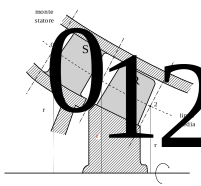
\includegraphics[width=.95\linewidth]{fig/SezioneTurbina.pdf}
  \captionof{figure}{}
  \label{fig:SezioneTurbina}
\end{minipage}%
\begin{minipage}{.5\textwidth}
  \centering
  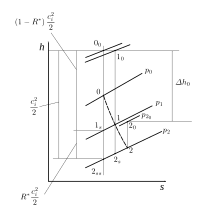
\includegraphics[width=.95\linewidth]{fig/hsturbine.pdf}
  \captionof{figure}{}
  \label{fig:hsturbine}
\end{minipage}
\end{figure}
\\Il salto entalpico tra i punti $1 - 2_s$ è leggermente superiore a quello presente tra i punti $1_s - 2_{ss}$ a causa della divergenza delle isobare. A tal proposito si introduce il fattore di recupero $f$. Questo fattore di recupero è fisicamente spiegabile dal fatto che la trasformazione, non essendo puramente isoentropica, causa un aumento della temperatura che verrà parzialmente recuperato nell'attraversamento successivo. 
\begin{center}
\begin{tabular}{l l l l l}
	$(1- R^*) \cdot \cfrac{c_i^2}{2}$ &&&& salto entalpico con espansione isoentropica\\
	$(1+f)R^* \cdot \cfrac{c_i^2}{2}$ &&&& salto entalpico tra $1$ e $2_s$\\
\end{tabular}
\end{center}
\subsection{Rendimenti}
Il rendimento è il seguente:
\begin{align*}
\eta = \cfrac{h_{0_0} - h_{2_0}}{h_{0_0} - h_{2_{ss}} - \Phi_E \cfrac{c_2^2}{2}} = \frac{\Delta h_0}{\Delta h_{is_{ts}}-\Phi_E \cfrac{c_2^2}{2}}
\end{align*}
con il termine $\Phi_E$ che rappresenta la quota cinetica a valle della turbina:
\begin{itemize}
	\item se $\Phi_E=1$ si considera un rendimento \textit{Total to Total} ($\eta \equiv \eta_{tt}$);
	\item se $\Phi_E=0$ si considera un rendimento \textit{Total to Static} ($\eta \equiv \eta_{ts}$).
\end{itemize}
Seguono ora una serie di definizioni:\\
\renewcommand\arraystretch{3}
\begin{tabular}{l l l l l}
	Coefficiente di portata: & & & &  $\Phi_1 = \cfrac{c_{m1}}{u_1}$\\
	Grado di reazione ideale: & & & & $R^* = \cfrac{h_{1s} - h_{2ss}}{h_{0_0} - h_{2_{ss}}} = \cfrac{\Delta h_{R_{is}}}{\Delta h_{is_{ts}}}$\\
	Energia cinetica totale: & & & &  $\cfrac{c_i^2}{2}=h_{0_0} - h_{2_{ss}}$\\
	Coefficiente di lavoro specifico ideale: & & & &  $\psi = \cfrac{h_{0_0} - h_{2_{ss}}}{\cfrac{u_1^2}{2}} = \cfrac{\Delta h_{is_{ts}}}{\cfrac{u_1^2}{2}}= \cfrac{c_i^2}{u_1^2}$\\
	Coefficiente di lavoro specifico reale: & & & &  $\lambda = \cfrac{h_{0_0} - h_{2_0}}{\cfrac{u_1^2}{2}}= \cfrac{\Delta h_0}{\cfrac{u_1^2}{2}}$\\
	Coefficiente di velocità periferica: & & & &  $k_{is} = \cfrac{u_1}{c_i} = \cfrac{1}{\sqrt{\psi}}$\\
\end{tabular}

\vspace{0.5cm}
Dopo aver adimensionalizzato i triangoli di velocità non è più possibile riferirsi ad una sola velocità meridiana in quanto questa diventa una grandezza di progettazione visto che definisce le sezioni della macchina; si usano quindi i rapporti tra velocità meridiane e tra i raggi:
\begin{align*}
\frac{c_{m2}}{c_{m1}} \;\; \text{e} \;\; \frac{r_2}{r_1}
\end{align*}
Si adimensionalizzano tutte le grandezze con la velocità periferica $u_1$. Chiaramente i triangoli di velocità saranno di dimensioni diverse come mostrato in figura \ref{fig:triangTurb}. 
\begin{figure}[h!]
\centering
  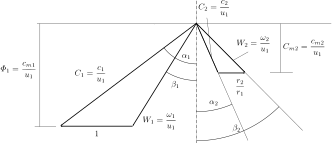
\includegraphics[width=.8\textwidth]{fig/triangTurb.pdf}
\caption{}
\label{fig:triangTurb}
\end{figure}
\\\'E possibile andare ora a sviluppare l'espressione del rendimento:
\begin{equation}
\eta = \cfrac{\Delta h_0}{\Delta h_{is_{ts}} - \Phi_E \cfrac{c_2^2}{2}} \cdot \frac{\frac{1}{u_1^2/2}}{\frac{1}{u_1^2/2}} = \frac{\lambda}{\psi - \Phi_E \left( C_2^2 \right)}
\end{equation}
con a numeratore
\begin{align*}
\lambda = \cfrac{\Delta h_0}{\cfrac{u_1^2}{2}} = \frac{2 \left( u_1 c_{u1} - u_2 c_{u2} \right)}{u_1^2} = 2 \bigg( C_{u1} - \frac{r_2}{r_1} C_{u2} \bigg)
\end{align*}
Si scrivono ora le velocità assolute adimensionalizzate, $C_i$, in funzione del rendimento e del grado di reazione:
\begin{align*}
\frac{c_1^2}{2} = \left( 1 - R^* \right) \frac{c_i^2}{2} \cdot \eta_s \;\;\;\; \Rightarrow \;\;\;\; c_1 = \sqrt{\eta_s \left( 1 - R^* \right)} \cdot c_i
\end{align*}
\begin{align*}
C_1 = \frac{c_1}{u_1} = \sqrt{\eta_s \left(1- R^* \right)} \cdot \frac{c_i}{u_1} \hspace{0.5cm} \mbox{con } \frac{c_i}{u_1} = \frac{1}{k_{is}}
\end{align*}
Risulta
\begin{equation}
\boxed{ C_1 = \frac{\sqrt{\eta_s}}{k_{is}} \sqrt{1 - R^*} }
\end{equation}
Si procede con la stessa operazione per le altre grandezze.

Per esprimere la velocità relativa adimensionalizzata $W_1$ si usa il teorema di Carnot:
\begin{align*}
W_1^2 = C_1^2 + 1^2 - 2 \cdot 1 \cdot C_1 \cos \cdot \big( \frac{\pi}{2} - \alpha_1 \big)
\end{align*}
ottenendo
\begin{equation}
\boxed{ W_1 = \sqrt{1 + \frac{\eta_{s}}{k_{is}^2} \left( 1 - R^* \right) - 2 \frac{\sqrt{\eta_s}}{k_{is}} \sqrt{1-R^*} \cdot \sin \alpha_1}}
\label{eq:W1}
\end{equation}

Per quanto riguarda $W_2$, si considera il salto entalpico e lo si esprime in funzione del fattore di recupero $f$:
\begin{equation}
h_2 - h_1 = \frac{u_2^2 - u_1^2}{2} - \frac{w_2^2 - w_1^2}{2}
\end{equation}
\begin{align*}
h_1 - h_2 = \frac{c_i^2}{2} \cdot R^* \left( 1 + f \right) \eta_R
\end{align*}
\begin{align*}
\Bigg[\frac{w_2^2 - w_1^2}{2} - \frac{u_2^2 - u_1^2}{2} = \frac{c_i^2}{2} \cdot R^* \left( 1 + f \right) \eta_R \Bigg] \cdot \frac{1}{u_1^2}
\end{align*}
\begin{equation}
\boxed{W_2 = \sqrt{\frac{\eta_R \left( 1 + f \right) R^*}{k_{is}^2} + \frac{\eta_s}{k_{is}^2}  \left(1 - R^* \right) - \frac{2 \sqrt{\eta_s}}{k_{is}} \sqrt{1 - R^*} \sin \alpha_1 + \bigg(\frac{r_2}{r_1} \bigg)^2 } }
\end{equation}
\\Per quanto riguarda $C_{m2}$:
\begin{align*}
c_{m2} = c_{m1} \frac{c_{m2}}{c_{m1}}=c_1 \cos \alpha_1 \cdot \frac{c_{m2}}{c_{m1}}
\end{align*}
\begin{align*}
C_{m2} = C_1 \cos \alpha_1 \cdot \frac{c_{m2}}{c_{m1}}
\end{align*}
ottenendo
\begin{equation}
\boxed{C_{m2} = \frac{c_{m2}}{c_{m1}} \frac{\sqrt{\eta_s}}{k_{is}} \sqrt{1 - R^*} \cos \alpha_1 }
\end{equation}
In questo modo è possibile scrivere il rendimento come funzionale di tutte le grandezze viste :
\begin{align*}
\boxed{\eta = f \bigg( \psi, \Phi_E, R^*, k_{is}, f, \frac{c_{m2}}{c_{m1}}, \frac{r_2}{r_1}, \alpha_1, \eta_s, \eta_R \bigg)}
\end{align*}
I primi quattro parametri sono parametri funzionali, $f$ dipende dalla divergenza delle isobare e quindi dalla natura del fluido, i tre parametri successivi sono parametri di progetto e infine gli ultimi due sono parametri della schiera rotorica e statorica.\\
\'E possibile tracciare un diagramma di rendimento Total to Static / Total to Total in funzione del coefficiente di lavoro specifico ideale (figura \ref{fig:Rendimenti_ts_tt}). 
\begin{figure}
\centering
  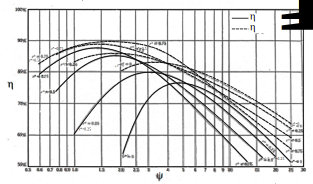
\includegraphics[width=.8\textwidth]{fig/Rendimenti_ts_tt.pdf}
\caption{}
\label{fig:Rendimenti_ts_tt}
\end{figure}
\section{Proprietà termodinamiche del flusso}
Si possono ora calcolare le proprietà termodinamiche del flusso nell'attraversamento della turbina. Si definisce il numero di Mach periferico come:
\begin{align*}
M_u = \frac{u_1}{a_{0_0}}
\end{align*}
\'E possibile esprimere la velocità acustica a monte della turbina in funzione dell'entalpia totale:
\begin{align*}
a_{0_0} = \sqrt{kRT_{0_0}} = \sqrt{\frac{c_p}{c_v} \left( c_p - c_v \right) T_{0_0}} = \sqrt{h_{0_0} \left( k - 1 \right)}
\end{align*}
e
\begin{align*}
\psi = \cfrac{h_{0_0} - h_{2ss}}{\cfrac{u_1^2}{2}} = \cfrac{\Delta h_{is_{ts}}}{\cfrac{u_1^2}{2}} = \cfrac{c_i^2}{u_1^2} \hspace{2cm} \frac{c_i^2}{2} = \psi \frac{u_1^2}{2} \cdot \frac{a_{0_0}^2}{a_{0_0}^2} = \frac{k-1}{2}\psi {M_u}^2 h_{0_0}
\end{align*}
Si ricavano quindi le espressioni dei punti delle trasformazioni isoentropiche:
\begin{align*}
h_{1s} = h_{0_0} - \left(1- R^* \right) \frac{c_i^2}{2} = h_{0_0} \bigg[ 1- \left( 1- R^* \right) \frac{k-1}{2} \psi M_u^2 \bigg]
\end{align*}
\begin{align*}
h_{2ss} = h_{0_0} - \frac{c_i^2}{2} = h_{0_0} \bigg[ 1 - \frac{k-1}{2} \psi M_u^2 \bigg]
\end{align*}
Ricordando che
\begin{align*}
\frac{c_1^2}{2} = \frac{c_i^2}{2} \left( 1- R^* \right) \eta_s
\end{align*}
si arriva alle espressioni dell'entalpia nei punti $1$ e $2$:
\begin{align*}
\boxed{h_1 = h_{0_0} - \frac{c_1^2}{2} = h_{0_0} \bigg[ 1- \left( 1- R^* \right) \frac{k-1}{2}  \psi M_u^2 \eta_s\bigg]}
\end{align*}
\begin{align*}
\boxed{h_2 = h_{0_0} - \Delta h_0 - \frac{c_2^2}{2} = h_{0_0} \bigg[ 1- \bigg( \eta_{ts} + \frac{C_2^2}{\psi} \bigg) \frac{k-1}{2} \psi M_u^2 \bigg]}
\end{align*}

\section{Schiere palari}
L'attraversamento del fluido attraverso la palettatura comporta una situazione meno critica dal punto di vista fluidodinamico rispetto il caso dei compressori. Il gradiente di pressione infatti, naturalmente non favorisce la separazione di vena fluida e perciò non sussistono grosse criticità sotto questo punto di vista permettendo di ottenere rendimenti più alti più facilmente. La deflessione imposta sarà quindi di gran lunga maggiore di quella del compressore e ne conseguiranno anche spessori maggiori. 
\begin{figure}
\centering
  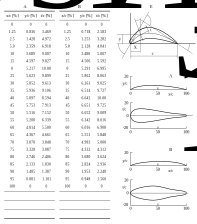
\includegraphics[width=\textwidth]{fig/SchierePaleTab.pdf}
\caption{}
\label{fig:SchierePaleTab}
\end{figure}

I profili a deflessione relativamente bassa, come quelli delle turbine a gas, si ricavano dalla somma di una distribuzione di spessori ad una linea media. Ci sono profili di diversa categoria e i valori sono ricavati in base a dei parametri di progettazione come mostrato in figura \ref{fig:SchierePaleTab}.

Nei profili ad alta deflessione, utilizzati soprattutto in macchine ad azione, la sezione è costituita da una carenatura ad arco di cerchio. Come si vede in figura \ref{fig:palaBassaDef}, la componente $w_1$ ha stesso modulo di $w_2$ e vi è semplicemente una deviazione nella direzione del secondo vettore. La palettatura è un arco di cerchio tangente alle due direzioni e presenta un inspessimento verso il centro per dare maggiore resistenza meccanica. La coda è tronca mentre il leading edge non può naturalmente esserlo e per questo viene arrotondato. 
\begin{figure}
\centering
  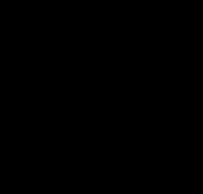
\includegraphics[width=.6\textwidth]{fig/palaBassaDef.pdf}
\caption{}
\label{fig:palaBassaDef}
\end{figure}

In alcuni casi, come con turbine a vapore, gli effetti di comprimibilità non sono trascurabili.\\
Come si può notare osservando la figura \ref{fig:SupSonic} in alto, nel caso sia presente un flusso subsonico si forma sul dorso del profilo isolato una zona supersonica con una discontinuità data da un'onda d'urto.\\
Osservando invece la figura \ref{fig:SupSonic} in basso, nel caso il flusso sia supersonico si verifica la formazione di un'onda d'urto prima del profilo isolato che porta quindi ad un incremento della sua resistenza al flusso; a valle si formano invece delle onde d'urto oblique.

Considerando un insieme di pale in presenza di velocità supersonica del flusso, figura \ref{fig:PaleSup} a destra, a valle del condotto convergente si instaura un'onda d'urto e un sistema di onde oblique che va ad interagire con la palettatura del rotore posta a valle. \'E possibile distinguere un'onda normale sul condotto (a) e un'onda obliqua a valle (b). Si tratta di un sistema complicato di onde d'urto. Per stabilizzare il comportamento della palettatura si utilizzerà quindi un leading edge appuntito.
\begin{figure}
\centering
\begin{minipage}{.5\textwidth}
  \centering
  \includegraphics[width=.95\linewidth]{fig/ou_schiera.png}
  \captionof{figure}{}
  \label{fig:ou_schiera}
\end{minipage}%
\begin{minipage}{.5\textwidth}
  \centering
  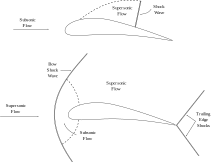
\includegraphics[width=.95\linewidth]{fig/SupSonic.pdf}
  \captionof{figure}{}
  \label{fig:SupSonic}
\end{minipage}
\end{figure}
\begin{figure}
\centering
  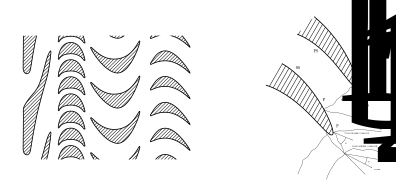
\includegraphics[width=\textwidth]{fig/PaleSup.pdf}
\caption{}
\label{fig:PaleSup}
\end{figure}

\section{Prestazioni della schiera}
Definiti i triangoli di velocità si cerca ora il coefficiente di perdita in uscita e l'angolo in uscita. In prima approssimazione si possono trascurare $Ma$ e $Re$.
\begin{figure}[h!]
\centering
  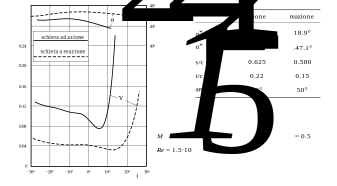
\includegraphics[width=\textwidth]{fig/PrestSchieraTurb.pdf}
\caption{}
\label{fig:PrestSchieraTurb}
\end{figure}

Stabilire l'angolo del fluido in uscita non è ovvio: in presenza di una deviazione elevata della palettatura è presente un ampio passo palare. Per definire l'angolo di deviazione in uscita si considera la normale al ventre del profilo dal trailing edge e il passo palare, figura \ref{fig:PrestSchieraTurb} in basso a destra, e quindi si ricava:
\begin{align*}
\alpha_2^* = \arccos \bigg(\cfrac{a}{s}\bigg)
\end{align*}
$\alpha_2$ è poco variabile al variare dell'incidenza; si rileva un comportamento abbastanza costante anche per il primo tratto del coefficiente di perdita.

\'E noto che l'angolo di flusso non sarà esattamente pari all'angolo di pala:
\begin{align*}
\cos \alpha_1 = \frac{1}{k} \cos \alpha_1^*
\end{align*}
dove $k$ può essere stimato con diverse correlazioni sperimentali. Un esempio di correlazione per il calcolo di $k$ è quella di \textit{Vaura}:
\begin{align*}
k = 1 - 10750 \bigg( \frac{t}{s} \bigg)^{3.3} \bigg( \frac{a}{s} \bigg)
\end{align*}
in cui $t$ è lo spessore della pala all'uscita.

Per quanto riguarda le perdite, è possibile considerare la cumulata delle diverse perdite come mostrato in figura \ref{fig:PerditeSchiera} oppure utilizzare alcune correlazioni. 
\begin{figure}
\centering
  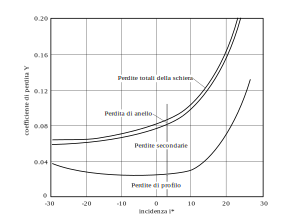
\includegraphics[width=.65\textwidth]{fig/PerditeSchiera.pdf}
\caption{}
\label{fig:PerditeSchiera}
\end{figure}
\subsection{Soderberg}
La correlazione di Soderberg permette di determinare globalmente tutte le perdite. \'E applicabile se vengono rispettate due condizioni:
\begin{itemize}
	\item la schiera si trova in condizioni di progetto;
	\item la solidità deve essere calcolata con un criterio di ottimizzazione (in particolare con il criterio di carico di Zweifel).
\end{itemize}
I coefficienti di perdita di energia adimensionalizzati rispetto l'energia cinetica effettiva allo scarico della schiera considerata sono:
\begin{align*}
\begin{cases}
\xi_1 = \cfrac{|h_1 - h_{1s}|}{\cfrac{1}{2} c_1^2} & \mbox{ per lo statore }\\
\\
\xi_2 = \cfrac{|h_2 - h_{2s}|}{\cfrac{1}{2} w_2^2} & \mbox{per il rotore }
\end{cases}
\end{align*}
Si cercano ora dei coefficienti funzione di:
\begin{itemize}
\item deflessione cinematica: $\Delta \alpha$ statore, $\Delta \beta$ rotore;
\item numero di Reynolds: $Re = \cfrac{D_i c_1 }{\nu}$
con $D_i$ diametro idraulico della sezione\footnote{ Diametro bagnato dal fluido: \begin{align*}
D_{i} = \frac{2 h s \cos \alpha_1}{h + s \cos \alpha_1} \mbox{ per lo statore}, \;\; D_{i} = \frac{2 h s \cos \beta_2}{h + s \cos \beta_2} \mbox{ per il rotore}
\end{align*} con $h$ altezza della pala.};
\item allungamento della pala $h/b$;
\item $t_{max}/c$.
\end{itemize}
Le correlazioni sono espresse rispetto ad una perdita $\xi^*$ (figura \ref{fig:Soderberg}) in funzione della deflessione cinematica $\varepsilon$ al variare del rapporto $t_{max}/c$. Si tratta di una sintesi di dati sperimentali di una palettatura di riferimento ricavati in galleria del vento.
\begin{align*}
\begin{cases}
\xi = \bigg( \cfrac{10^5}{Re} \bigg)^{0.25} \bigg[ \left( 1 + \xi^* \right) \bigg ( 0.975 + 0.075 \cfrac{h}{b} \bigg) -1 \bigg] & \mbox{per lo statore} \\
\xi = \bigg( \cfrac{10^5}{Re} \bigg)^{0.25} \bigg[ \left( 1 + \xi^* \right) \bigg ( 0.993 + 0.021 \cfrac{h}{b} \bigg) -1 \bigg] & \mbox{per il rotore}
\end{cases}
\end{align*}
\begin{figure}
\centering
  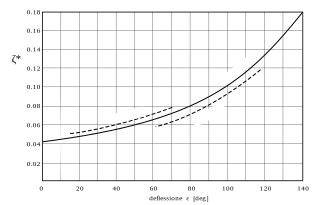
\includegraphics[width=\textwidth]{fig/Soderberg.pdf}
\caption{}
\label{fig:Soderberg}
\end{figure}
\subsection{Ainley-Mathieson}
Si possono vedere anche altre correlazioni come quella di Ainley-Mathieson per la valutazione delle perdite di profilo. Si definiscono dei parametri fissi:
\begin{itemize}
\item $Re = 2 \cdot 10^5$ (basato sulla corda)
\item $M_1 < 0.6$
\item $t_{max}/c = 0.2$
\item $t/s = 0.02$
\item Condizioni nominali (angolo di incidenza nullo)
\end{itemize}
Si definisce il coefficiente di perdita di pressione totale come:
\begin{align*}
Y_P = \frac{p_{0_0} - p_{1_0}}{p_{1_0} - p_1}
\end{align*}
Sperimentalmente la perdita di profilo è definita come:
\begin{align*}
Y_P = \big[ Y_P^* + m_a^2 \left( Y_P^{**} - Y_P^* \right) \big] \Biggl(\frac{\frac{t_{max}}{c}}{0.2} \Biggr)^{m_a}
\end{align*}
con $Y_P^*$ e $Y_P^{**}$ due coefficienti di perdita valutati in due classiche configurazioni di pale:
\begin{align*}
Y_P^* \;\; \to \;\;
\begin{cases}
\alpha_0 = 0\\
R = 0\\
m_a = 0
\end{cases} \hspace{2.5cm}
Y_P^{**} \;\; \to \;\;
\begin{cases}
\alpha_1 = -\alpha_0\\
R = 0.5\\
m_a = 1
\end{cases}
\end{align*}
\begin{align*}
m_a = - \frac{\alpha_0}{\alpha_1} \hspace{1.5cm} 0.15 \leq \frac{t_{max}}{c} \leq 0.25
\end{align*}
\begin{figure}
\centering
  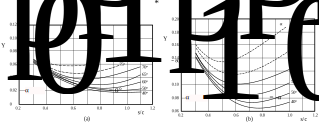
\includegraphics[width=\textwidth]{fig/Mathieson.pdf}
\caption{Perdite di profilo secondo Ainley e Mathieson per ugelli (a) e pale ad azione (b), in condizioni standard.}
\label{fig:Mathieson}
\end{figure}
\\Si possono quindi esprimere le correlazioni corrette:\\
\begin{tabular}{l l}
	$ Y_P = Y_{P,0.02} \bigg[ 1 + 7 \bigg( \frac{t}{s} - 0.02 \bigg) \bigg] $ & correlazione per spessore uscita diverso da quello standard\\
	$ Y_P = Y_{P,2 \cdot 10^5} \bigg( \frac{2 \cdot 10^5}{Re} \bigg)^{0.2} $ &  correlazione per Re diverso da quello standard\\
\end{tabular}

\vspace{0.5cm}
La precedente correlazione fornisce l'espressione solamente per le perdite di profilo; a queste dovranno essere aggiunte le perdite secondarie e per giochi:
\begin{align*}
Y_S + Y_G = \Big( \lambda + B \frac{\delta}{k} \Big) \Bigg( \frac{c_L}{\frac{s}{c}} \frac{\cos^2 \alpha_1}{\cos^3 \alpha_{\infty}} \Bigg)
\end{align*}
con
\begin{itemize}
\item $B = 0.5$ per pale ``libere", $B = 0.25$ per pale ``cerchiate";
\item $h$ altezza della pala;
\item $\delta$ gioco radiale;
\item $\lambda$ un coefficiente sperimentale in funzione di $\Theta$ secondo il grafico \ref{fig:lambdaPerditeSchiera}. $\Theta$ è definito come:
\end{itemize}
\begin{align*}
\Theta = \cfrac{\bigg(\cfrac{A_1}{A_0}\bigg)^2}{1- \cfrac{D_i}{D_e}}
\end{align*}
\begin{figure}
\centering
  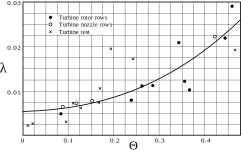
\includegraphics[width=.6\textwidth]{fig/lambdaPerditeSchiera.pdf}
\caption{}
\label{fig:lambdaPerditeSchiera}
\end{figure}

In questo modo si vanno quindi a calcolare le perdite in condizioni fuori progetto usando correlazioni come quelle riportate in figura \ref{fig:FuoriProgT1}.
\begin{figure}
\centering
  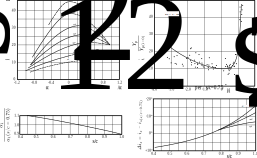
\includegraphics[width=\textwidth]{fig/FuoriProgT1.pdf}
\caption{}
\label{fig:FuoriProgT1}
\end{figure}

\section{Criteri di carico}
\begin{figure}[h!]
\centering
  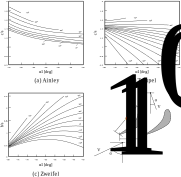
\includegraphics[width=0.95\textwidth]{fig/Ainley.pdf}
\caption{}
\label{fig:Ainley}
\end{figure}
Una volta determinata la schiera è opportuno verificare con un criterio di carico se la solidità scelta è sostenibile o meno. Per esempio con molte pale aumentano le perdite perché aumenta la superficie bagnata ma per contro si riesce a realizzare meglio la variazione d'angolo che è quella che da momento alla turbina.\\
In figura \ref{fig:Ainley} sono illustrati i diversi criteri di carico. I criteri di Zweifel impongono un vincolo sul rapporto tra forza tangenziale e una forza tangenziale ideale:
\begin{align*}
\cfrac{F_t}{F_{t,id}} = \cfrac{F_t}{\cfrac{1}{2} \rho b c_1^2} = c_{F_t} = 2 \cos^2 \alpha_1 \bigg(\cfrac{c_{m0}}{c_{m1}} \tan \alpha_0 - \tan \alpha_1 \bigg) \cfrac{s}{b} = 0.8
\end{align*}
In figura \ref{fig:CritCaricoT} è rappresentata in rosso l'area formata dall'andamento delle pressioni ideali nell'attraversamento del fluido nel canale interpalare; viene poi evidenziata l'area formata dall'andamento reale in grigio scuro. Il loro rapporto è appunto il rapporto tra le forze tangenziali.
\begin{figure}[h!]
\centering
  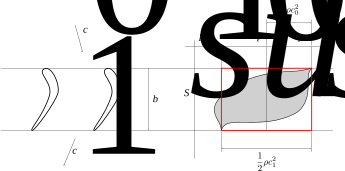
\includegraphics[width=0.95\textwidth]{fig/CritCaricoT.pdf}
\caption{}
\label{fig:CritCaricoT}
\end{figure}

\chapter{Compressori assiali}

\section{Introduzione}
I compressori assiali sono macchine relativamente recenti, si tratta di una macchina nata nel dopoguerra come componente per i gruppi turbina a gas in campo aeronautico. I primi motori aeronautici costituiti da gruppo turbogas sono stati inizialmente costruiti come compressori radiali. C'è una forte correlazione tra compressione ottenibile e rendimento, oggi qualsiasi turbogas salvo eccezioni specifiche si utilizzano compressori assiali. 
\begin{figure}[h!]
\centering
  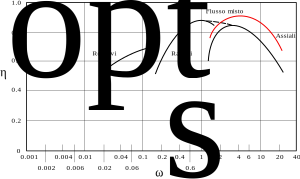
\includegraphics[width=.8\textwidth]{fig/PrestComp.pdf}
\caption{A destra le curve di rendimento per le macchine assiali. Si nota l'evidente aumento delle prestazioni (in rosso) rispetto alle prime macchine}
\label{fig:PrestComp}
\end{figure}
Nel diagramma in figura \ref{fig:PrestComp} è presente il rendimento del compressore in funzione della velocità specifica (che ricordiamo essere la caratteristica di macchina). Si nota che all'aumentare della velocità specifica si va verso macchine assiali, fino ad un certo punto della storia le macchine assiali non hanno goduto di rendimenti competitivi. In rosso è presentata la curva dello stato attuale dei rendimenti per macchine assiali. 
\begin{figure}
\centering
  \includegraphics[width=.5\textwidth]{fig/hsComp.png}
\caption{1: ingresso statore 2: uscita statore - entrata rotore 3: uscita statore.}
\label{fig:hsComp}
\end{figure}
Nel diagramma termodinamico in figura \ref{fig:hsComp} sono riportati gli stati di rierimento di uno stadio di compressore assiale. Nella parte rotorica avviene il lavoro con un relativo aumento della velocità mentre nello c'è il recupero in termini di pressione. Nello studio della macchina assiale vengono fatte generalmente le seguenti assunzioni:
\begin{itemize}
\item Flusso adiabatico;
\item Stadio ``normale" o ``ripetuto": tutti gli stadi hanno gli stessi profili
\begin{align*}
c_1 = c_2 \Rightarrow h_3-h_1 = h_{03} - h_{01}
\end{align*}
\item Velocità assiale costante (coincide con la velocità meridiana)
\begin{align*}
c_{m1} = c_{m2}
\end{align*}
\item densità costante nello stadio
\begin{align*}
\rho = cost. 
\end{align*}
\end{itemize}
\begin{align*}
\omega_s = \cfrac{\sqrt{\phi}}{\psi^{3/4}} \cdot \sqrt{\bigg( \cfrac{D_e}{D_i} \bigg)^2 -1}
\end{align*}
\begin{align*}
\phi = \frac{Q}{u \cdot S}
\end{align*}
\begin{align*}
\psi = \cfrac{\Delta h_{0is}}{\cfrac{u^2}{2}}
\end{align*}
\section{Lavoro e triangoli di velocità}
Nel rotore si conserva la rotalpia
\begin{equation}
h_1 + \frac{1}{2} w_1^2 = h_2 + \frac{1}{2} w_2^2
\end{equation}
Nello statore si conserva l'entalpia
\begin{equation}
h_2 + \frac{1}{2} c_2^2 = h_3 + \frac{1}{2} c_3^2
\end{equation}
Il lavoro scambiato è quello che avviene nella parte rotorica, definiamo un parametro adimensionale per quest'ultimo
\begin{equation}
\lambda = \frac{u \cdot c_{u2} - u \cdot c_{u1}}{u^2} = \frac{c_{u2} - c_{u1}}{u}
\end{equation}
\begin{figure}
\centering
  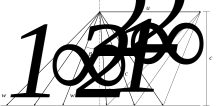
\includegraphics[width=.9\textwidth]{fig/triangComp.pdf}
\caption{}
\label{fig:triangComp}
\end{figure}
L'obiettivo è quello di determinare la relazione tra $\lambda$ e cifra di portata $\Phi$. Vado a disegnare i triangoli di velocità relativi allo stadio elementare come mostrato in figura \ref{fig:triangComp}. Ricordo che per definizione la componente meridiana e periferica sono costanti. Posso scrivere le seguenti tre relazioni 
\begin{align*}
c_{u2} = u - w_{u2}
\end{align*}
\begin{align*}
w_{u2} = c_m \tan \beta_2
\end{align*}
\begin{align*}
c_{u1} = c_m \tan \alpha_1
\end{align*}
Posso quindi scrivere
\begin{align*}
\lambda = 1- \frac{w_{u2}}{u} - \frac{c_{u1}}{u} = 1 - \frac{c_m}{u} \left(\tan \beta_2 + \tan \alpha_1 \right)
\end{align*}
Ma definendo  la cifra di portata come
\begin{align*}
\Phi = \frac{c_m}{u}
\end{align*}
Posso finalmente scrivere la cifra di flusso in funzione della cifra di portata, la caratteristica teorica del nostro compressore
\begin{equation}
\lambda = 1 - \Phi \left( \tan \beta_2 + \tan \alpha_1 \right) = 1 - k \cdot \Phi
\end{equation}
Con $k$ costante che dipende dalla geometria della macchina. Si tratta di una rappresentazione molto simile a quella nel caso delle pompe centrifuche nelle quali a seconda del valore di $k$ si ha la curva caratteristica della pompa; questo viene chiarito meglio dal diagramma in figura \ref{fig:CondProg}.
\begin{figure}
\centering
  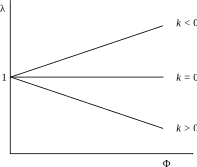
\includegraphics[width=.4\textwidth]{fig/CondProg.pdf}
\caption{}
\label{fig:CondProg}
\end{figure}
Andiamo ora a definire una condizione particolare di progetto ``lambda design"$\lambda_d$.
\begin{align*}
\lambda_d = 1 - k \cdot \Phi_d, \;\; k = f(\lambda_d,\Phi_d)
\end{align*}
Calcolo ora il rapporto $\lambda/\lambda_d$:
\begin{equation} \label{eq:lambdad}
\frac{\lambda}{\lambda_d} = \frac{1}{\lambda_d} - \frac{\Phi}{\Phi_d} \Bigg( \frac{1-\lambda_d}{\lambda_d} \Bigg), \;\;\; 0.3 < \lambda_d < 0.4
\end{equation}
Si tratta di una famiglia di rette, in figura \ref{fig:LambdaPhiChart} è rappresentato il diagramma caratteristico però in termini di rapporti rispetto alle condizioni di progetto. Si vede che nel caso ideale di $\lambda_d = 1$ il lavoro scambiato sarebbe indipendente dalla portata, sarebbe una situazione abbastanza attraente. 
\begin{figure}
\centering
\begin{minipage}{.5\textwidth}
  \centering
  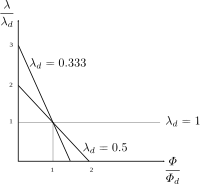
\includegraphics[width=.9\linewidth]{fig/LambdaPhiChart.pdf}
  \captionof{figure}{}
  \label{fig:LambdaPhiChart}
\end{minipage}%
\begin{minipage}{.5\textwidth}
  \centering
  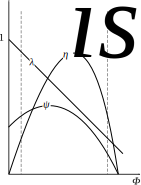
\includegraphics[width=.9\linewidth]{fig/CarattReal.pdf}
  \captionof{figure}{}
  \label{fig:CarattReal}
\end{minipage}
\end{figure}
Generalmente in un compressore, infatti, la pressione di output è definita mentre la portata è regolata, $\lambda_d = 1$ avrei una macchina perfetta, il rapporto di pressione lo riuscirei sempre a mantenere e basta che regoli la portata per ottenere la pressione voluta. Purtroppo non è così perchè le palettature non si comportano in modo ideale, si hanno separazioni di vela, inspessimenti di strato limite... dal punto di vista realistico si riesce ad ottenere un $\lambda_d$ definito come nell'equazione \ref{eq:lambdad}. 

Come mostrato in figura \ref{fig:CarattReal} otterrò un comportamento non ideale che non avrà andament rettilineo, avrtò quindi un campo di utilizzo essendo limitato sia a portate basse che a portate alte. 

Caratteristica reale:
\begin{equation}
\psi = \frac{\Delta h_{0is}}{u^2} = \lambda \cdot \eta_{is}, \;\;\; \Delta h_{0is} = h_{30is} - h_{10}
\end{equation}

Non abbiamo ancora detto nulla riguardo la forma della pala in funzione del grado di reazione\footnote{Che ricordiamo essere il rapporto tra il salto entalpico elaborato tra parte rotorica e statorica}. 
\begin{align*}
R = \frac{h_2 - h_1}{h_3-h_1} 
\end{align*}
Sapendo che
\begin{align*}
\begin{rcases*}
c_{u2} = u - w_{u2}\\
c_{u1} = u - w_{u1}
\end{rcases*}
\Rightarrow c_{u2} - c_{u1} = w_{u1} - w_{u2} 
\end{align*}
Vado a sviluppare il grado di reazione della macchina applicando la conservazione della rotalpia al numeratore e l'espressione del lavoro euleriano al denominatore:
\begin{align*}
R = \frac{w_1^2 - w_2^2}{2 u (c_{u2} - c_{u1})} &= \frac{(w_{u1} + w_{u2})\cancel{(w_{u1}-w_{u2})}}{2 u \cancel{(c_{u2} - c_{u1})}} =\\
&= \frac{w_{u1} + w_{u2}}{2u} = \\
&= \frac{c_m \left(\tan \beta_1 + \tan \beta_2 \right)}{2 u}
\end{align*}
Definendo poi
\begin{align*}
\tan \beta_{\infty} = \frac{\tan \beta_1 + \tan \beta_2}{2}, \;\; \Phi = \frac{c_m}{u}
\end{align*}
Si ottiene
\begin{equation}
\boxed{R = \Phi \tan \beta_{\infty} = \frac{w_{u \infty}}{u}}
\end{equation}
Lo stesso risultato poteva essere raggiunto nel seguente modo
\begin{equation}
w_{u1} = u - c_{u1} \; \Rightarrow \; R = \frac{1}{2} + \frac{\tan \beta_2 - \tan \alpha_1}{2} \cdot \Phi \simeq \frac{1}{2} + cost \cdot \Phi
\end{equation}
Quello che è importante notare è che:
\begin{align*}
R = 0.5 \to \beta_2 = \alpha_1
\end{align*}
Il grado di reazione è costante con la portata e la palettatura sarà simmetrica.

Per rappresentare lo stadio al variare del grado di reazione andiamo per prima cosa a definire i triangoli di velocità come si vede in figura \ref{fig:StadioRipetuto}.
\begin{figure}
\centering
  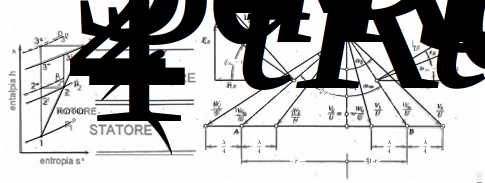
\includegraphics[width=\textwidth]{fig/StadioRipetuto.pdf}
\caption{}
\label{fig:StadioRipetuto}
\end{figure}
Sempre facendo riferimento alla figura posso quindi scrivere
\begin{align*}
r \cdot \tan \beta_{\infty} = R 
\end{align*}
\begin{align*}
\lambda = \cfrac{\Delta h_0}{\cfrac{u^2}{2}} = \cfrac{u \Delta c_u}{\cfrac{u^2}{2}} = \cfrac{2 \Delta c_u}{u} = \cfrac{2 \Delta w_u}{u}
\end{align*}
\begin{align*}
\frac{\Delta c_u}{u} = \frac{\Delta w_u}{u} = \frac{\lambda}{2}
\end{align*}
Qual'ora si operi un cambio di portata vediamo che gli unici angoli che si conservano sono $\beta_2$ e $\alpha_1$, la cifra si flusso passa dalle condizioni di design $\Phi_d$ alle condizioni generiche $\Phi$ come si vede in figura \ref{fig:CondFuoriProg}.
\begin{figure}
\centering
  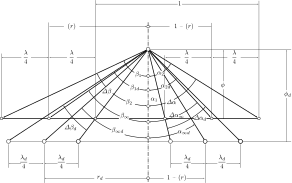
\includegraphics[width=\textwidth]{fig/CondFuoriProg.pdf}
\caption{}
\label{fig:CondFuoriProg}
\end{figure}

Possiamo classificare alcune condizioni notevoli riportate in figura \ref{fig:ComprAssTab}.
\begin{figure}
\centering
  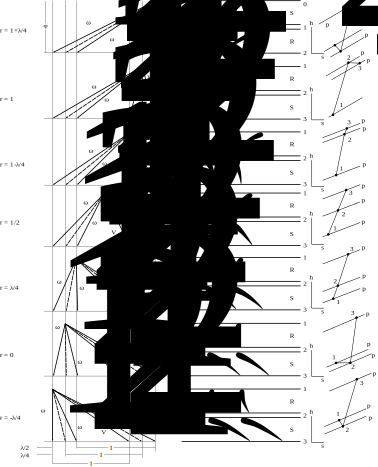
\includegraphics[width=1.2\textwidth]{fig/ComprAssTab.pdf}
\caption{}
\label{fig:ComprAssTab}
\end{figure}
Il primo caso con $r = 1 + \lambda /4$ è particolare in quanto si ha grado di reazione maggiore di uno, lo statore precede infatti il rotore. Mi ritrovo con una velocità di uscita puramente assiale.

Con grado di reazione $r = 1$ le velocità assolute ingresso uscita sono simmetriche.

Con $r = 1 - \lambda/4$ la velocità assoluta è puramente assiale, mentre quella allo scarico non lo è. 

Sono poi rappresentate le geometrie per gradi di reazione sempre più ridotti. 

La soluzione $r = 1/2$ è la più diffusa e utilizzata eccetto per il primo e l'ultimo stadio in cui si vogliono distribuzioni di velocità particolari, velicità assoluta in uscita e poi in ingresso puramente assiale. In questa configurazione si avranno profili uguali ma specchiati, l'intervallo p1 p3 è poi diviso equamente in due parti uguali tra la parte statorica e la parte rotorica. 

\section{Termodinamica}
Vediamo il calcolo del rendimento al variare della portata e del grado di reazione. Partiamo dalla definizione di rendimento isoentropico
\begin{align*}
\eta_{is} = \frac{\Delta h_{is}}{\Delta h_0} = \frac{\Delta p}{\rho \cdot \Delta h_0}
\end{align*}
Dal primo principio:
\begin{align*}
T ds = dh - \frac{dp}{\rho}
\end{align*}
ma
\begin{align*}
ds = 0 \Rightarrow dh = \frac{dp}{\rho}
\end{align*}
Otteniamo quindi
\begin{equation}\label{eq:etadp}
\eta_{is} = \frac{\Delta p}{\rho \cdot \Delta h_0} = \cfrac{\Delta p}{\rho \cdot \cfrac{\lambda}{2} u^2}
\end{equation}
L'incremento di pressione totale si può però ulteriormente sviluppare come somma di incremento di pressione sviluppato nel rotore e nello statore
\begin{align*}
\Delta p = \Delta p_R + \Delta p_S = \frac{F_{aR}}{s_R} + \frac{F_{aS}}{s_S} = \frac{F_{tR} \cdot \tan(\beta_{\infty} - \varepsilon_R)}{s_R} + \frac{F_{tS} \cdot \tan(\alpha_{\infty} - \varepsilon_S)}{s_S}
\end{align*}
Con $\varepsilon_S, \; \varepsilon_R$\footnote{Per quanto riguarda i pedici "s" sta per statore, "r" per rotore.} indice di efficienza del profilo.
Possiamo fare qualche assunzione. I profili hanno drag molto più piccolo del lift quindi
\begin{align*}
\tan \varepsilon_R \simeq \varepsilon_R = \frac{D_R}{L_R} \;\;\;\;\; \tan \varepsilon_S \simeq \varepsilon_S = \frac{D_S}{L_S}
\end{align*}
Utilizzando le componenti di forza del triangolo di velocità si ottiene
\begin{align*}
F_{tR} = \dot{m} \Delta w_u = \overbrace{s_R \cdot \rho \cdot c_m}^\text{$ \dot{m} $} \cdot \overbrace{\lambda \cdot u \cdot \frac{1}{2}}^\text{$\Delta w_u$}  
\end{align*}
Analogamente riesco a fare la stessa cosa per la parte statorica
\begin{align*}
F_{tS} = \dot{m} \Delta c_m = s_S \cdot \rho \cdot \lambda \cdot \Phi \cdot u^2 \cdot \frac{1}{2}
\end{align*}
Andando a sostituire
\begin{align*}
\Delta p = \frac{1}{2} \rho \lambda u^2 \big[ \Phi \tan \left( \beta_{\infty} - \varepsilon_R \right) + \Phi \tan \left( \alpha_{\infty} - \varepsilon_S \right) \big] 
\end{align*}
Ricordando le relazioni
\begin{align*}
R = \Phi \tan \beta_{\infty}
\end{align*}
\begin{align*}
1 - R = \Phi \tan \alpha_{\infty} 
\end{align*}
\begin{align*}
\tan ( \beta_{\infty} - \varepsilon_R ) = \frac{\tan \beta_{\infty} - \tan \varepsilon_R}{1 + \tan \beta_{\infty} \tan \varepsilon_R} \simeq \frac{\tan \beta_{\infty} - \varepsilon_R}{1 + \tan \beta_{\infty} \cdot \varepsilon_R}
\end{align*}
\begin{align*}
\tan (\alpha_{\infty} - \varepsilon_S) \simeq \frac{\tan \alpha_{\infty} - \varepsilon_S}{1 + \tan \alpha_{\infty} \cdot \epsilon_S}
\end{align*}
Ottengo in fine la relazione del salto di pressione in funzione del grado di reazione e di $\lambda$:
\begin{equation}
\Delta p = \frac{1}{2} \rho \lambda u^2 \Bigg[ \frac{R - \varepsilon_R \Phi}{\Phi + \varepsilon_R R} + \frac{1 - R - \varepsilon_S \Phi}{\Phi + \varepsilon_S (1-R)} \Bigg] \cdot \Phi
\end{equation}
Posso dire che epsilon r è circa epsilon s. Il rendimento isoentropico ricordando l'equazione \ref{eq:etadp} diviene:
\begin{equation}
\boxed{ \eta_{is} = \Bigg[ \frac{R - \varepsilon_R \Phi}{\Phi + \varepsilon_R R} + \frac{1 - R - \varepsilon_S \Phi}{\Phi + \varepsilon_S (1-R)} \Bigg] \cdot \Phi }
\end{equation}
Cerco ora il coefficiente di reazione
\begin{align*}
\varepsilon_S \simeq \varepsilon_R = cost = \varepsilon
\end{align*}
\begin{align*}
\frac{d \eta_{is}}{dR} = 0 \Rightarrow R_{opt} = 0.5 per \forall \Phi
\end{align*}
\begin{align*}
\eta_{|R= 0.5} = 2 \Phi \cdot \frac{1- 2 \varepsilon \Phi}{\varepsilon + 2 \Phi}
\end{align*}
Si ha quindi $R_{opt} = 0.5$. 
Naturalmente si vede che il rendimento del compressore è migliorato alla diminuzione di $\varepsilon$.
\begin{align*}
\frac{d\eta_{|R=0.5}}{d \Phi} = 0 \Rightarrow \Phi_{opt} = \frac{1}{2} \left( \sqrt{1 + \varepsilon^2} - \varepsilon \right) \simeq \frac{1 - \varepsilon}{2}
\end{align*}
Determino ora il rendimento ottimale in funzione di $\Phi$
\begin{equation}
\eta_{max} = 1 + 2 \varepsilon^2 - 2 \varepsilon \sqrt{1 + \varepsilon^2} \simeq 1 - 2 \varepsilon \left( 1 - \varepsilon \right)
\end{equation}
\begin{figure}
\centering
  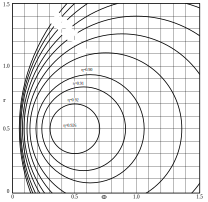
\includegraphics[width=\textwidth]{fig/IsoRendCompAss.pdf}
\caption{Curve isorendimento di uno stadio assiale in funzione del grado di reazione e coefficiente di portata per efficienza del profilo assegnata}
\label{}
\end{figure}

\section{Progettazione della schiera}
\subsection{Correlazioni di Howell}
Sono presenti molteplici correlazioni per progettare una macchina assiale. Noi vedremo un filone di correlazioni, sono datate ma non hanno perso di validità. Anche nella progettazione di una nuova macchina è utile partire da un predimensionamento per poi andare a raffinare con strumenti moderni. Verrà quindi usato come passo preliminare.
Si parte dalle seguenti riflessioni:
\begin{itemize}
\item La deflessione imposta alla corrente è limitata: nell'ordine delle decine di gradi (20, 30 al massimo 40);
\item Profili sottili a bassa curvatura.
\end{itemize}
Le perdite possono quindi essere suddivise in 
\begin{itemize}
\item Perdite di anello;
\item perdite di profilo;
\item perdite per flussi secondari.
\end{itemize}
La perdita di profilo è direttamente correlata al $c_D$, sarà quella in cui si può andare maggiormente a lavorare. 
Il flusso all'interno del compressore è un moto elicoidale. Il flusso lambisce la cassa della macchina, vi sarà quindi un attrito tra fluido e la partete, queste perdite le chiameremo perdite di ``anello".
Le perdite per flussi secondari sono state adeguatamente trattate nel capitolo precedente. 
Si andrà quindi a lavorare sulle perdite di profilo aggiungendo poi le altre due perdite tramite coefficienti di correlazione.

Le perdite di anello inducono un drag aggiuntivo correlato a quanto più è elevato lo sviluppo radiale della pala, definito $H$ lo sviluppo radiale e $s$ passo palare, si può scrivere
\begin{align*}
C_{Da} = 0.02 \cdot \frac{s}{H}
\end{align*}
Abbiamo poi che la perdita per flussi secondari è correlata con il quadrato del coefficiente di portanza, quanto più io ho una portanza elevata quanto più impongo una deviazione, tanto più è probabile che abbia un instaurarsi di moti secondari.
\begin{align*}
C_{Da} = 0.018 \cdot C_L^2
\end{align*}
Posso andare quindi a scrivere un coefficiente di resistenza complessivo
\begin{align*}
C_{Dtot} = C_D + C_{Da} + C_{Ds} = C_D + 0.02 \cdot \frac{s}{H} + 0.018 \cdot C_L^2
\end{align*}
In figura \ref{fig:ComprStageLoss} si vede come le varie perdite inficiano sull'efficienza della schiera.
\begin{figure}
\centering
  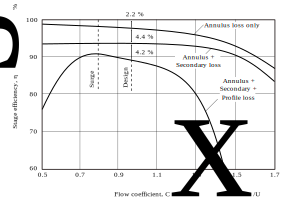
\includegraphics[width=\textwidth]{fig/ComprStageLoss.pdf}
\caption{}
\label{fig:ComprStageLoss}
\end{figure}
La progettazione preliminare con la correlazione di Howell, si va a cercare la relazione tra gli angoli geometrici in ingresso e uscita e gli angoli che deve avere il fluido. La prima correlazione di Howell dice che la condizione di riferimento, ovvero la deflessione che la corrente subisce nell'attraversamento delle pale (nominale) $\varepsilon^*$ viene riferita rispetto alla deviazione di stallo $\varepsilon_s$
\begin{equation}
\varepsilon^* = 0.8 \cdot \varepsilon_s
\end{equation}
In figura \ref{fig:Howell} è rappresentato l'andamento della deflessione in funzione dell'angolo di incidenza. Come si nota un tratto pressocchè lineare seguito da un brusco cambiamento di curvatura. Quest'ultimo è facilmente individuabile, risutlta quindi comodo utilizzarlo come punto di riferimento per individuare la deflessione nominale. Cpme deflessione nominale si utilizzarà quindi un valore che va a minimizzare le perdite, tenendo conto poi dei margini di operabilità.  
\begin{figure}
\centering
  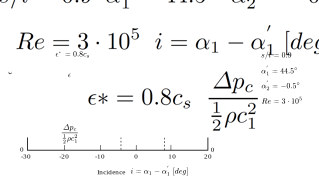
\includegraphics[width=\textwidth]{fig/Howell.pdf}
\caption{}
\label{fig:Howell}
\end{figure}
In figura \ref{fig:SchieraDim} si riportano le nomenclature utilizzate in questo capitolo, è rappresentata la differenza tra angoli geometrici e fluidodinamici.
\begin{figure}
\centering
  \includegraphics[width=\textwidth]{fig/SchieraDim.pdf}
\caption{}
\label{fig:SchieraDim}
\end{figure}
La prima correlazione di Howell permette di calcolare gli angoli del flusso attesi da una chiera di data solidità ($\varepsilon = \varepsilon*$).
La seconda correlazione di Howell permette di trovare, noti gli angoli di flusso, i corrispondenti valori degli angoli geometrici della schiera ($\varepsilon = \varepsilon*$).
La terza correlazione di Howell permette di calcolare le prestazioni in off-design, quando $\varepsilon \neq \varepsilon*$ 
In figura \ref{fig:1CorrHowell} è rappresentata la prima correlazione di Howell al variare della solidità della schiera. Si nota che a parità di deflessine nominalre si avrà una maggiore angolo in uscira per schiere più compatte.
\begin{figure}
\centering
  \includegraphics[width=.4\textwidth]{fig/1CorrHowell.pdf}
\caption{}
\label{fig:1CorrHowell}
\end{figure}
Si definisce il campo di validità della relazione
\begin{align*}
\varepsilon^* = f \bigg( \frac{s}{l}, \alpha_2^*, Re \bigg) \;\; 20^{\circ} < \theta < 40^{\circ}
\end{align*}
\begin{align*}
\varepsilon^* = f\bigg(\frac{s}{l}, \alpha_2*\bigg)\;\; Re > 3 \cdot 10^5
\end{align*}
La deflessione nominale è definita come segue
\begin{align*}
\varepsilon^* = \alpha_1^* - \alpha_2^*
\end{align*}
Le curve espresse come relazione tra gli angoli
\begin{align*}
\tan \alpha_1^* - \tan \alpha_2^* = \cfrac{1.55}{1 + 1.5 \cfrac{s}{l}}
\end{align*}
La seconda correlazione di Howell mi da il valore della deviazione $\delta$, lo scostamento tra angolo geometrico e angolo effettivo del flusso in uscita. Si ha che $\delta$ dipende dai seguenti fattori
\begin{align*}
\delta = f \bigg( \theta, forma \; della \; pala, \frac{s}{l}, \gamma \bigg)
\end{align*}
Si usa la seguente relazione
\begin{align*}
\delta^* = m \theta \bigg( \frac{s}{l} \bigg)^n
\end{align*}
con $n = 1/2$ per schiere di compressore e $n = 1$ per schiere di IGV. Il coefficiente $m$ è funzione della forma della pala, si ripete che queste sono correlazioni approssimative.
\begin{align*}
m = 0.23 \cdot \bigg( 2 \cdot \frac{a}{l} \bigg)^2 + \frac{\alpha_2^*}{500}
\end{align*}
Con queste correlazioni posso ridurre i gradi di libertà nella definizione della geometria. Infatti una volta scelti $ \theta, \sigma $, dalla seconda correlazione ottengo $ \delta^* $ e dalla prima corrlazione trovo $ \varepsilon^* $. In questo modo posso definire
\begin{align*}
i^* = \varepsilon^* - \theta + \delta^*
\end{align*}
\begin{align*}
\alpha_{1g} = \alpha_1^* - i^*
\end{align*}
\begin{align*}
\alpha_{1g} = \alpha_2^* - \delta^*
\end{align*}
Ora posso effettivamente disegnare la schiera. 

\subsection{Condizioni fuori progetto}
Si utilizzano delle ulteriori relazioni nelle quali si va a rapportare la deflessione relativa $\varepsilon/\varepsilon^*$ rispetto alle altre caratteristiche (figura \ref{fig:FuoriProg1})
\begin{figure}
\centering
  \includegraphics[width=\textwidth]{fig/FuoriProg1.pdf}
\caption{}
\label{fig:FuoriProg1}
\end{figure}
Queste relazioni sono state ricavati per numeri di Mach bassi, vediamo cosa succede aumentando la velocità e quindi avvicinandosi alle condizioni soniche. In figura \ref{fig:FuoriProg2} si rapporta il coefficiente di pressione In il numero di Mach in entrata. 
\begin{figure}
\centering
\begin{minipage}{.6\textwidth}
  \centering
  \includegraphics[width=.95\linewidth]{fig/FuoriProg2.pdf}
  \captionof{figure}{}
  \label{fig:FuoriProg2}
\end{minipage}%
\begin{minipage}{.4\textwidth}
  \centering
  \includegraphics[width=.95\linewidth]{fig/FuoriProgMach.pdf}
  \captionof{figure}{ Campo di pressione attorno al profilo al variare del numero di Mach}
  \label{fig:FuoriProgMach}
\end{minipage}
\end{figure}
Il diagramma è riferito a condizioni specifiche. Di divide la curva in due parti da $M_C$, oltre questo Mach critico l'andamento delle pressioni sul singolo profilo, Fintanto che $ M < M_C$ l'andamento è quello mostrato in figura. Al crescere di $M$ il campo di pressione attorno al profilo si modifica con la possibile formazione di un'onda d'urto, il recupero di pressione varia anch'esso in maniera sensibile perggiorando le prestazioni del profilo. Nella condizione di $ M_{max} $ si ha un'onda d'urto che occupa l'intero condotto, sono in chocking e la portata non può variare.
\begin{figure}
\centering
  \includegraphics[width=.4\textwidth]{fig/FuoriProg3.pdf}
\caption{}
\label{fig:FuoriProg3}
\end{figure}
In figura \ref{fig:FuoriProg3} ho le relazioni che mi correlano deflessione della schiera e rendimento in funzione di una grandezza dipendente da $M$ completamente definita una volta definiti $M_C$ e $M_{max}$ che ricordiamo essere specifici per condizioni fissate; soprattutto $M_C$ è pesantemente influenzato dall'angolo di incidenza come si vede in figura \ref{fig:FuoriProg4}.
\begin{figure}
\centering
  \includegraphics[width=.4\textwidth]{fig/FuoriProg4.pdf}
\caption{}
\label{fig:FuoriProg4}
\end{figure}

\subsection{Criterio di carico}
Al variare del numero di pale, a parità di lavoro svolto dalla macchina dovrò imporre diverse deflessioni, ne conseguirà un carico diverso sulla singola pala. Con poche pale dovrò infatti imporre deflessioni maggiori con un forte carico sul singolo profilo.
Si va a fare una verifica, fissata la schiera e la solidità si va a calcolare il coefficiente di deflessione locale $D_{loc}$ che dice quant'è la massima decelerazione a cui è soggetta la schiera (eq. \ref{eq:D_loc}). Si considera poi la riduzione di quantità di moto come nell'equazione \ref{eq:D_ridqmot} integrando sullo spessore occupato dalla scia, con $V$ è velocità di riferimento mentre $\nu$ è la velocità come funzione della posizione.
\begin{figure}
\centering
  \includegraphics[width=\textwidth]{fig/CritCarico1.pdf}
\caption{}
\label{fig:CritCarico1}
\end{figure}
Fattore di diffusione locale
\begin{equation}\label{eq:D_loc}
D_{loc} = \frac{V_{max} - V_2}{V_{max}}
\end{equation}
\begin{equation}\label{eq:D_ridqmot}
\theta = \int_{\delta_P}^{\delta_S} \frac{\nu}{V} \bigg(1- \frac{\nu}{V} \bigg) dy
\end{equation} 
\begin{figure}
\centering
  \includegraphics[width=.4\textwidth]{fig/CritCarico2.pdf}
\caption{}
\label{fig:CritCarico2}
\end{figure}
Se ho molte pale, l'integrale diventa molto grande perchè potrei avere l'intero canale palare occupato dalla scia, quindi come criterio empirico utilizzo
\begin{align*}
\frac{\theta}{c} < 0.2
\end{align*}
In questo modo l'inspessimento di strato limite è considerato trascurabile rispetto alla corrente principale. 
\begin{figure}
\centering
  \includegraphics[width=\textwidth]{fig/CritCarico3.pdf}
\caption{}
\label{fig:CritCarico3}
\end{figure}
Il valore di $D$ si può calcolare anche attraverso differenti correlazioni (figura \ref{fig:CritCarico3})
\begin{align*}
D = \bigg( \frac{V_1 - V_2}{V_1} \bigg) + \bigg( \frac{V_{t1} - V_{t2}}{2 \sigma V_1} \bigg) = \bigg( 1 - \frac{\cos \alpha_1}{cos \alpha_2} \bigg) + \frac{\cos \alpha_1}{2 \sigma} (\tan \alpha_1 - \tan \alpha_2)
\end{align*}
e come criterio empirico si usa $$ D \leqslant 0.4 \div 0.5  $$
\begin{figure}
\centering
  \includegraphics[width=.4\textwidth]{fig/CritCarico4.pdf}
\caption{}
\label{fig:CritCarico4}
\end{figure}
Infine si possono andare a cercare correlazioni rispetto allo strato limite come mostrato in figura \ref{fig:CritCarico4} ma ciò non ha molto senso in quanto nel contesto moderno è propio la parte di progettazione che si effettua per via numerica. 
\begin{align*}
\Delta M = \int_0^{\delta} \rho u dy (U-u) = \rho \int_0^{\delta} u (U-u) dy
\end{align*} 
Spessore della quantità di moto dello strato limite
\begin{equation}
\theta = \frac{\Delta M}{\rho U^2} = \int_0^{\delta} \frac{u}{U} \bigg( 1 -\frac{u}{U} \bigg) dy
\end{equation}

\section{Schiere supersoniche}
Fin'ora abbiamo parlato di schiere di copressori con deflusso subsonico debolmente comprimibile con rapporti di compressione modesti (10 - 20 peerc) partendo dal presupposto che il flusso in ingresso sia inferiore alla velocità sonica. Quindi 
\begin{align*}
\begin{cases}
M_1 <1\\
M_2 <1
\end{cases}
\end{align*} 
Vediamo delle condizioni diverse. Si parlerà di compressore transonico se 
\begin{align*}
\begin{cases}
M_1 >1\\
M_2 <1
\end{cases}
\end{align*} 
Nel caso in cui si arrivi in condizione soniche all'interno della macchina si faranno ulteriori distinzioni rispetto alla componente assiale: per $M_{1a} < 1 $ si parlerà di \textit{regime innescato} o \textit{non innescato} mentre per $ M_{1a} > 1 $ si parlerà di \textit{regime saturo}.
Ulteriori possibilità che non hanno però rilevanza nei compressori sono 
\begin{align*}
\begin{cases}
M_1 <1\\
M_2 >1
\end{cases}
\end{align*} 
In questo caso il flusso viene accelerato ma per definizione in un compressore cerco esattamente l'effetto opposto. Si ha poi
\begin{align*}
\begin{cases}
M_1 >1\\
M_2 >1
\end{cases}
\end{align*} 
in cui il flusso è interamente supersonico, non ha interessi applicativi.

Le schiere supersoniche trovano applicazioni particolari in campo aeronautico. Nel regime non innescato notiamo che è presente un'onda d'urto normale al flusso, si avrà una zona supersonica a monte della schiera, l'aumento di velocità naturalmente è dovuto all'aumento di spessore della schiera.

Nel regime innescato la perturbazione di pressione occupa integralmente il condoto palare, distinguo in maniera chiara, la portata è bloccata. 

In regime saturo la componente assiale è superiore a 1, il blocco sonico è a monte della schiera, a monte si creano onde oblique che dissipano energia.

\begin{figure}[h!]
\centering
  \includegraphics[width=.8\textwidth]{fig/Schlieren1.pdf}
\caption{}
\label{fig:Schlieren1}
\end{figure}
\begin{figure}[h!]
\centering
  \includegraphics[width=.8\textwidth]{fig/Schlieren2.png}
\caption{}
\label{fig:Schlieren2}
\end{figure}
Questo tipo di deflusso consente un salto di pressione più elevato a scapito però di una pesante perdita in termini di rendimento. 


%\include{chapter}
%\appendix
%\include{appendix}

\backmatter%%%%%%%%%%%%%%%%%%%%%%%%%%%%%%%%%%%%%%%%%%%%%%%%%%%%%%%
%\include{Contenuto/solutions_it}
%%%%%%%%%%%%%%%%%%%%%%%%% referenc_it.tex %%%%%%%%%%%%%%%%%%%%%%%%%%%%%%
% Esempio di referenze
%
%
% Usare questo file come template per il vostro documento.
%
%%%%%%%%%%%%%%%%%%%%%%%% Springer-Verlag %%%%%%%%%%%%%%%%%%%%%%%%%%

%
% Utenti BibTeX: usare
% \bibliographystyle{}
% \bibliography{}
%
% Non-utenti BibTeX: usare
\begin{thebibliography}{[KLR73]}
%
% ed usare \bibitem per creare referenze.
%
% Usare la sintassi ed il markup seguenti per le vostre referenze.
%
% Monografie
\bibitem[KLR73]{monograph} Kagan, A.M., Linnik, Y.V., Rao, C.R.:
Characterization Problems in Mathematical Statistics. Wiley, New York (1973)

% Contributed Works
\bibitem[Mey89]{contribution} Meyer, P.A.: A short presentation of
stochastic calculus. In: Emery, M. (ed) Stochastic Calculus in
Manifolds. Springer, Berlin Heidelberg New York (1989)

% Journal
\bibitem[MR97]{journal} Miller, B.M., Runggaldier, W.J.: Kalman
filtering for linear systems with coefficients driven by a hidden Markov
jump process. Syst. Control Lett., \textbf{31}, 93--102 (1997)

% Tesi
\bibitem[Ros77]{thesis} Ross, D.W.: Lysosomes and storage diseases. MA
Thesis, Columbia University, New York (1977)

\end{thebibliography}

%\printindex

%%%%%%%%%%%%%%%%%%%%%%%%%%%%%%%%%%%%%%%%%%%%%%%%%%%%%%%%%%%%%%%%%%%%%%

\end{document}





